\documentclass[twoside]{book}

% Packages required by doxygen
\usepackage{fixltx2e}
\usepackage{calc}
\usepackage{doxygen}
\usepackage[export]{adjustbox} % also loads graphicx
\usepackage{graphicx}
\usepackage[utf8]{inputenc}
\usepackage{makeidx}
\usepackage{multicol}
\usepackage{multirow}
\PassOptionsToPackage{warn}{textcomp}
\usepackage{textcomp}
\usepackage[nointegrals]{wasysym}
\usepackage[table]{xcolor}

% Font selection
\usepackage[T1]{fontenc}
\usepackage[scaled=.90]{helvet}
\usepackage{courier}
\usepackage{amssymb}
\usepackage{sectsty}
\renewcommand{\familydefault}{\sfdefault}
\allsectionsfont{%
  \fontseries{bc}\selectfont%
  \color{darkgray}%
}
\renewcommand{\DoxyLabelFont}{%
  \fontseries{bc}\selectfont%
  \color{darkgray}%
}
\newcommand{\+}{\discretionary{\mbox{\scriptsize$\hookleftarrow$}}{}{}}

% Page & text layout
\usepackage{geometry}
\geometry{%
  a4paper,%
  top=2.5cm,%
  bottom=2.5cm,%
  left=2.5cm,%
  right=2.5cm%
}
\tolerance=750
\hfuzz=15pt
\hbadness=750
\setlength{\emergencystretch}{15pt}
\setlength{\parindent}{0cm}
\setlength{\parskip}{3ex plus 2ex minus 2ex}
\makeatletter
\renewcommand{\paragraph}{%
  \@startsection{paragraph}{4}{0ex}{-1.0ex}{1.0ex}{%
    \normalfont\normalsize\bfseries\SS@parafont%
  }%
}
\renewcommand{\subparagraph}{%
  \@startsection{subparagraph}{5}{0ex}{-1.0ex}{1.0ex}{%
    \normalfont\normalsize\bfseries\SS@subparafont%
  }%
}
\makeatother

% Headers & footers
\usepackage{fancyhdr}
\pagestyle{fancyplain}
\fancyhead[LE]{\fancyplain{}{\bfseries\thepage}}
\fancyhead[CE]{\fancyplain{}{}}
\fancyhead[RE]{\fancyplain{}{\bfseries\leftmark}}
\fancyhead[LO]{\fancyplain{}{\bfseries\rightmark}}
\fancyhead[CO]{\fancyplain{}{}}
\fancyhead[RO]{\fancyplain{}{\bfseries\thepage}}
\fancyfoot[LE]{\fancyplain{}{}}
\fancyfoot[CE]{\fancyplain{}{}}
\fancyfoot[RE]{\fancyplain{}{\bfseries\scriptsize Generated by Doxygen }}
\fancyfoot[LO]{\fancyplain{}{\bfseries\scriptsize Generated by Doxygen }}
\fancyfoot[CO]{\fancyplain{}{}}
\fancyfoot[RO]{\fancyplain{}{}}
\renewcommand{\footrulewidth}{0.4pt}
\renewcommand{\chaptermark}[1]{%
  \markboth{#1}{}%
}
\renewcommand{\sectionmark}[1]{%
  \markright{\thesection\ #1}%
}

% Indices & bibliography
\usepackage{natbib}
\usepackage[titles]{tocloft}
\setcounter{tocdepth}{3}
\setcounter{secnumdepth}{5}
\makeindex

% Hyperlinks (required, but should be loaded last)
\usepackage{ifpdf}
\ifpdf
  \usepackage[pdftex,pagebackref=true]{hyperref}
\else
  \usepackage[ps2pdf,pagebackref=true]{hyperref}
\fi
\hypersetup{%
  colorlinks=true,%
  linkcolor=blue,%
  citecolor=blue,%
  unicode%
}

% Custom commands
\newcommand{\clearemptydoublepage}{%
  \newpage{\pagestyle{empty}\cleardoublepage}%
}

\usepackage{caption}
\captionsetup{labelsep=space,justification=centering,font={bf},singlelinecheck=off,skip=4pt,position=top}

%===== C O N T E N T S =====

\begin{document}

% Titlepage & ToC
\hypersetup{pageanchor=false,
             bookmarksnumbered=true,
             pdfencoding=unicode
            }
\pagenumbering{roman}
\begin{titlepage}
\vspace*{7cm}
\begin{center}%
{\Large vivalib library }\\
\vspace*{1cm}
{\large Generated by Doxygen 1.8.11}\\
\end{center}
\end{titlepage}
\clearemptydoublepage
\tableofcontents
\clearemptydoublepage
\pagenumbering{arabic}
\hypersetup{pageanchor=true}

%--- Begin generated contents ---
\chapter{Hierarchical Index}
\section{Class Hierarchy}
This inheritance list is sorted roughly, but not completely, alphabetically\+:\begin{DoxyCompactList}
\item \contentsline{section}{\+\_\+\+W\+D\+IR}{\pageref{struct___w_d_i_r}}{}
\item \contentsline{section}{\+\_\+wdirent}{\pageref{struct__wdirent}}{}
\item \contentsline{section}{viva\+:\+:Batch\+Processor}{\pageref{classviva_1_1_batch_processor}}{}
\item \contentsline{section}{viva\+:\+:Buffered\+Channel$<$ Data $>$}{\pageref{classviva_1_1_buffered_channel}}{}
\item \contentsline{section}{D\+IR}{\pageref{struct_d_i_r}}{}
\item \contentsline{section}{dirent}{\pageref{structdirent}}{}
\item \contentsline{section}{viva\+:\+:Files}{\pageref{classviva_1_1_files}}{}
\item \contentsline{section}{viva\+:\+:Input}{\pageref{classviva_1_1_input}}{}
\begin{DoxyCompactList}
\item \contentsline{section}{viva\+:\+:Image\+List\+Input}{\pageref{classviva_1_1_image_list_input}}{}
\item \contentsline{section}{viva\+:\+:Video\+Input}{\pageref{classviva_1_1_video_input}}{}
\end{DoxyCompactList}
\item \contentsline{section}{viva\+:\+:Keyboard\+Listener}{\pageref{classviva_1_1_keyboard_listener}}{}
\begin{DoxyCompactList}
\item \contentsline{section}{viva\+:\+:Batch\+Process\+Frame}{\pageref{classviva_1_1_batch_process_frame}}{}
\item \contentsline{section}{viva\+:\+:Process\+Frame}{\pageref{classviva_1_1_process_frame}}{}
\end{DoxyCompactList}
\item \contentsline{section}{viva\+:\+:Keys}{\pageref{structviva_1_1_keys}}{}
\item \contentsline{section}{viva\+:\+:Mouse\+Listener}{\pageref{classviva_1_1_mouse_listener}}{}
\begin{DoxyCompactList}
\item \contentsline{section}{viva\+:\+:Batch\+Process\+Frame}{\pageref{classviva_1_1_batch_process_frame}}{}
\item \contentsline{section}{viva\+:\+:Process\+Frame}{\pageref{classviva_1_1_process_frame}}{}
\end{DoxyCompactList}
\item \contentsline{section}{viva\+:\+:Output}{\pageref{classviva_1_1_output}}{}
\begin{DoxyCompactList}
\item \contentsline{section}{viva\+:\+:Image\+Output}{\pageref{classviva_1_1_image_output}}{}
\item \contentsline{section}{viva\+:\+:None\+Output}{\pageref{classviva_1_1_none_output}}{}
\item \contentsline{section}{viva\+:\+:Video\+Output}{\pageref{classviva_1_1_video_output}}{}
\end{DoxyCompactList}
\item \contentsline{section}{viva\+:\+:Process\+Input}{\pageref{classviva_1_1_process_input}}{}
\item \contentsline{section}{viva\+:\+:Processor}{\pageref{classviva_1_1_processor}}{}
\item \contentsline{section}{viva\+:\+:Process\+Output}{\pageref{classviva_1_1_process_output}}{}
\item \contentsline{section}{viva\+:\+:thread\+\_\+guard}{\pageref{classviva_1_1thread__guard}}{}
\end{DoxyCompactList}

\chapter{Class Index}
\section{Class List}
Here are the classes, structs, unions and interfaces with brief descriptions\+:\begin{DoxyCompactList}
\item\contentsline{section}{\hyperlink{struct___w_d_i_r}{\+\_\+\+W\+D\+IR} }{\pageref{struct___w_d_i_r}}{}
\item\contentsline{section}{\hyperlink{struct__wdirent}{\+\_\+wdirent} }{\pageref{struct__wdirent}}{}
\item\contentsline{section}{\hyperlink{classviva_1_1_batch_process_frame}{viva\+::\+Batch\+Process\+Frame} }{\pageref{classviva_1_1_batch_process_frame}}{}
\item\contentsline{section}{\hyperlink{classviva_1_1_batch_processor}{viva\+::\+Batch\+Processor} }{\pageref{classviva_1_1_batch_processor}}{}
\item\contentsline{section}{\hyperlink{classviva_1_1_buffered_channel}{viva\+::\+Buffered\+Channel$<$ Data $>$} }{\pageref{classviva_1_1_buffered_channel}}{}
\item\contentsline{section}{\hyperlink{struct_d_i_r}{D\+IR} }{\pageref{struct_d_i_r}}{}
\item\contentsline{section}{\hyperlink{structdirent}{dirent} }{\pageref{structdirent}}{}
\item\contentsline{section}{\hyperlink{classviva_1_1_files}{viva\+::\+Files} }{\pageref{classviva_1_1_files}}{}
\item\contentsline{section}{\hyperlink{classviva_1_1_image_list_input}{viva\+::\+Image\+List\+Input} }{\pageref{classviva_1_1_image_list_input}}{}
\item\contentsline{section}{\hyperlink{classviva_1_1_image_output}{viva\+::\+Image\+Output} }{\pageref{classviva_1_1_image_output}}{}
\item\contentsline{section}{\hyperlink{classviva_1_1_input}{viva\+::\+Input} }{\pageref{classviva_1_1_input}}{}
\item\contentsline{section}{\hyperlink{classviva_1_1_keyboard_listener}{viva\+::\+Keyboard\+Listener} }{\pageref{classviva_1_1_keyboard_listener}}{}
\item\contentsline{section}{\hyperlink{structviva_1_1_keys}{viva\+::\+Keys} }{\pageref{structviva_1_1_keys}}{}
\item\contentsline{section}{\hyperlink{classviva_1_1_mouse_listener}{viva\+::\+Mouse\+Listener} }{\pageref{classviva_1_1_mouse_listener}}{}
\item\contentsline{section}{\hyperlink{classviva_1_1_none_output}{viva\+::\+None\+Output} }{\pageref{classviva_1_1_none_output}}{}
\item\contentsline{section}{\hyperlink{classviva_1_1_output}{viva\+::\+Output} }{\pageref{classviva_1_1_output}}{}
\item\contentsline{section}{\hyperlink{classviva_1_1_process_frame}{viva\+::\+Process\+Frame} }{\pageref{classviva_1_1_process_frame}}{}
\item\contentsline{section}{\hyperlink{classviva_1_1_process_input}{viva\+::\+Process\+Input} }{\pageref{classviva_1_1_process_input}}{}
\item\contentsline{section}{\hyperlink{classviva_1_1_processor}{viva\+::\+Processor} }{\pageref{classviva_1_1_processor}}{}
\item\contentsline{section}{\hyperlink{classviva_1_1_process_output}{viva\+::\+Process\+Output} }{\pageref{classviva_1_1_process_output}}{}
\item\contentsline{section}{\hyperlink{classviva_1_1thread__guard}{viva\+::thread\+\_\+guard} }{\pageref{classviva_1_1thread__guard}}{}
\item\contentsline{section}{\hyperlink{classviva_1_1_video_input}{viva\+::\+Video\+Input} }{\pageref{classviva_1_1_video_input}}{}
\item\contentsline{section}{\hyperlink{classviva_1_1_video_output}{viva\+::\+Video\+Output} }{\pageref{classviva_1_1_video_output}}{}
\end{DoxyCompactList}

\chapter{Class Documentation}
\hypertarget{struct___w_d_i_r}{}\section{\+\_\+\+W\+D\+IR Struct Reference}
\label{struct___w_d_i_r}\index{\+\_\+\+W\+D\+IR@{\+\_\+\+W\+D\+IR}}


Collaboration diagram for \+\_\+\+W\+D\+IR\+:
\nopagebreak
\begin{figure}[H]
\begin{center}
\leavevmode
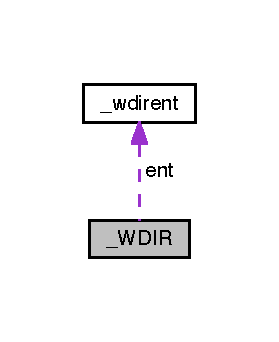
\includegraphics[width=134pt]{struct___w_d_i_r__coll__graph}
\end{center}
\end{figure}
\subsection*{Public Attributes}
\begin{DoxyCompactItemize}
\item 
struct \hyperlink{struct__wdirent}{\+\_\+wdirent} {\bfseries ent}\hypertarget{struct___w_d_i_r_a84ae1457352005f813ed4b3dc1994b62}{}\label{struct___w_d_i_r_a84ae1457352005f813ed4b3dc1994b62}

\item 
W\+I\+N32\+\_\+\+F\+I\+N\+D\+\_\+\+D\+A\+T\+AW {\bfseries data}\hypertarget{struct___w_d_i_r_a065b17b666ee06c4e8068d8accb0eef9}{}\label{struct___w_d_i_r_a065b17b666ee06c4e8068d8accb0eef9}

\item 
int {\bfseries cached}\hypertarget{struct___w_d_i_r_a9b7432df163d1e291ba5925347fd4af3}{}\label{struct___w_d_i_r_a9b7432df163d1e291ba5925347fd4af3}

\item 
H\+A\+N\+D\+LE {\bfseries handle}\hypertarget{struct___w_d_i_r_a694510e166fd3e797b3e15b9e4b3810a}{}\label{struct___w_d_i_r_a694510e166fd3e797b3e15b9e4b3810a}

\item 
wchar\+\_\+t $\ast$ {\bfseries patt}\hypertarget{struct___w_d_i_r_a700ff3a1096fb36452c571b0f55b4e60}{}\label{struct___w_d_i_r_a700ff3a1096fb36452c571b0f55b4e60}

\end{DoxyCompactItemize}


The documentation for this struct was generated from the following file\+:\begin{DoxyCompactItemize}
\item 
dirent\+V\+S.\+h\end{DoxyCompactItemize}

\hypertarget{struct__wdirent}{}\section{\+\_\+wdirent Struct Reference}
\label{struct__wdirent}\index{\+\_\+wdirent@{\+\_\+wdirent}}
\subsection*{Public Attributes}
\begin{DoxyCompactItemize}
\item 
long {\bfseries d\+\_\+ino}\hypertarget{struct__wdirent_ac8cfaf294a0b6a49287d3f384c280c93}{}\label{struct__wdirent_ac8cfaf294a0b6a49287d3f384c280c93}

\item 
unsigned short {\bfseries d\+\_\+reclen}\hypertarget{struct__wdirent_aff7f360608e576cd18cf11f2caf13ef3}{}\label{struct__wdirent_aff7f360608e576cd18cf11f2caf13ef3}

\item 
size\+\_\+t {\bfseries d\+\_\+namlen}\hypertarget{struct__wdirent_a0050d6131e6fa90206903e216b38799e}{}\label{struct__wdirent_a0050d6131e6fa90206903e216b38799e}

\item 
int {\bfseries d\+\_\+type}\hypertarget{struct__wdirent_a3c3874604ffccbeeaffd96709763cc3b}{}\label{struct__wdirent_a3c3874604ffccbeeaffd96709763cc3b}

\item 
wchar\+\_\+t {\bfseries d\+\_\+name} \mbox{[}P\+A\+T\+H\+\_\+\+M\+AX\mbox{]}\hypertarget{struct__wdirent_a267f915cd36cad5969337a9192cab567}{}\label{struct__wdirent_a267f915cd36cad5969337a9192cab567}

\end{DoxyCompactItemize}


The documentation for this struct was generated from the following file\+:\begin{DoxyCompactItemize}
\item 
dirent\+V\+S.\+h\end{DoxyCompactItemize}

\hypertarget{classviva_1_1_batch_process_frame}{}\section{viva\+:\+:Batch\+Process\+Frame Class Reference}
\label{classviva_1_1_batch_process_frame}\index{viva\+::\+Batch\+Process\+Frame@{viva\+::\+Batch\+Process\+Frame}}


{\ttfamily \#include $<$viva.\+h$>$}



Inheritance diagram for viva\+:\+:Batch\+Process\+Frame\+:
\nopagebreak
\begin{figure}[H]
\begin{center}
\leavevmode
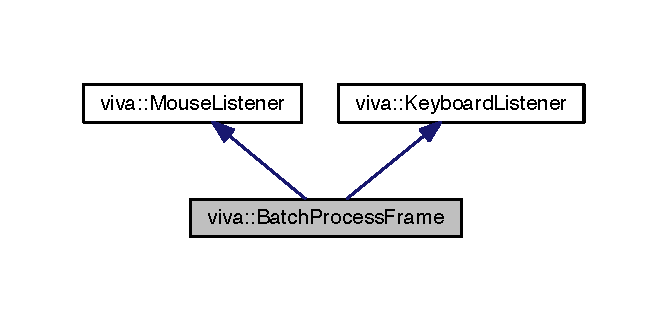
\includegraphics[width=320pt]{classviva_1_1_batch_process_frame__inherit__graph}
\end{center}
\end{figure}


Collaboration diagram for viva\+:\+:Batch\+Process\+Frame\+:
\nopagebreak
\begin{figure}[H]
\begin{center}
\leavevmode
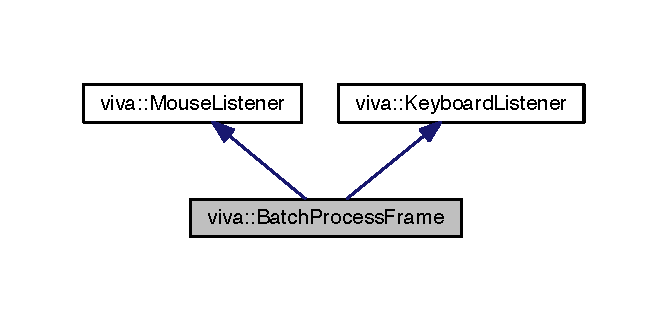
\includegraphics[width=320pt]{classviva_1_1_batch_process_frame__coll__graph}
\end{center}
\end{figure}
\subsection*{Public Member Functions}
\begin{DoxyCompactItemize}
\item 
{\bfseries Batch\+Process\+Frame} (const size\+\_\+t count=10)\hypertarget{classviva_1_1_batch_process_frame_a126f3b1c309eaeac244b761df7d921c0}{}\label{classviva_1_1_batch_process_frame_a126f3b1c309eaeac244b761df7d921c0}

\item 
virtual size\+\_\+t {\bfseries batch\+Process\+Size} ()\hypertarget{classviva_1_1_batch_process_frame_a1c9c59bc1d59d62e890271867ba23321}{}\label{classviva_1_1_batch_process_frame_a1c9c59bc1d59d62e890271867ba23321}

\item 
virtual void {\bfseries operator()} (size\+\_\+t frameN, const vector$<$ Mat $>$ \&frames, Mat \&output)\hypertarget{classviva_1_1_batch_process_frame_acfcb93fe2954cb748bc7c436864a8e49}{}\label{classviva_1_1_batch_process_frame_acfcb93fe2954cb748bc7c436864a8e49}

\item 
virtual void \hyperlink{classviva_1_1_batch_process_frame_a70b9f91a0d9fadb04ec4db3df7fbd2a8}{mouse\+Input} (int event, int x, int y, int flags)
\item 
virtual void \hyperlink{classviva_1_1_batch_process_frame_a7b4b1dbd173e0d900e7d1461c373fdad}{left\+Button\+Down} (int x, int y, int flags)
\item 
virtual void \hyperlink{classviva_1_1_batch_process_frame_ab7b8be0c726713cbf8be004ed9974ec6}{right\+Button\+Down} (int x, int y, int flags)
\item 
virtual void \hyperlink{classviva_1_1_batch_process_frame_a34fc0aff605d24a0260f466cd386c091}{middle\+Button\+Down} (int x, int y, int flags)
\item 
virtual void \hyperlink{classviva_1_1_batch_process_frame_afaf81db14d5a7f6f97c766498c9b66c9}{mouse\+Move} (int x, int y, int flags)
\item 
virtual void \hyperlink{classviva_1_1_batch_process_frame_a956265d099d3b4f4305045bfccceb308}{keyboard\+Input} (int key)
\end{DoxyCompactItemize}
\subsection*{Protected Attributes}
\begin{DoxyCompactItemize}
\item 
size\+\_\+t {\bfseries \+\_\+count}\hypertarget{classviva_1_1_batch_process_frame_ac0c401ebf80e5346d0e376279eb46c3f}{}\label{classviva_1_1_batch_process_frame_ac0c401ebf80e5346d0e376279eb46c3f}

\end{DoxyCompactItemize}


\subsection{Detailed Description}
Batch Process Frame. Process batchs of specific size from the input at once. 

\subsection{Member Function Documentation}
\index{viva\+::\+Batch\+Process\+Frame@{viva\+::\+Batch\+Process\+Frame}!keyboard\+Input@{keyboard\+Input}}
\index{keyboard\+Input@{keyboard\+Input}!viva\+::\+Batch\+Process\+Frame@{viva\+::\+Batch\+Process\+Frame}}
\subsubsection[{\texorpdfstring{keyboard\+Input(int key)}{keyboardInput(int key)}}]{\setlength{\rightskip}{0pt plus 5cm}virtual void viva\+::\+Batch\+Process\+Frame\+::keyboard\+Input (
\begin{DoxyParamCaption}
\item[{int}]{key}
\end{DoxyParamCaption}
)\hspace{0.3cm}{\ttfamily [inline]}, {\ttfamily [virtual]}}\hypertarget{classviva_1_1_batch_process_frame_a956265d099d3b4f4305045bfccceb308}{}\label{classviva_1_1_batch_process_frame_a956265d099d3b4f4305045bfccceb308}
It will be called only when the user stroke a keyboard key 
\begin{DoxyParams}{Parameters}
{\em key} & the value of the pressed key \\
\hline
\end{DoxyParams}


Reimplemented from \hyperlink{classviva_1_1_keyboard_listener_a903947e765f8130cfe1b3ce882c95998}{viva\+::\+Keyboard\+Listener}.

\index{viva\+::\+Batch\+Process\+Frame@{viva\+::\+Batch\+Process\+Frame}!left\+Button\+Down@{left\+Button\+Down}}
\index{left\+Button\+Down@{left\+Button\+Down}!viva\+::\+Batch\+Process\+Frame@{viva\+::\+Batch\+Process\+Frame}}
\subsubsection[{\texorpdfstring{left\+Button\+Down(int x, int y, int flags)}{leftButtonDown(int x, int y, int flags)}}]{\setlength{\rightskip}{0pt plus 5cm}virtual void viva\+::\+Batch\+Process\+Frame\+::left\+Button\+Down (
\begin{DoxyParamCaption}
\item[{int}]{x, }
\item[{int}]{y, }
\item[{int}]{flags}
\end{DoxyParamCaption}
)\hspace{0.3cm}{\ttfamily [inline]}, {\ttfamily [virtual]}}\hypertarget{classviva_1_1_batch_process_frame_a7b4b1dbd173e0d900e7d1461c373fdad}{}\label{classviva_1_1_batch_process_frame_a7b4b1dbd173e0d900e7d1461c373fdad}
It will be called only when a mouse left click is triggered 

Reimplemented from \hyperlink{classviva_1_1_mouse_listener_ae2b6952da67ea99e47f5fcfa2e1780c7}{viva\+::\+Mouse\+Listener}.

\index{viva\+::\+Batch\+Process\+Frame@{viva\+::\+Batch\+Process\+Frame}!middle\+Button\+Down@{middle\+Button\+Down}}
\index{middle\+Button\+Down@{middle\+Button\+Down}!viva\+::\+Batch\+Process\+Frame@{viva\+::\+Batch\+Process\+Frame}}
\subsubsection[{\texorpdfstring{middle\+Button\+Down(int x, int y, int flags)}{middleButtonDown(int x, int y, int flags)}}]{\setlength{\rightskip}{0pt plus 5cm}virtual void viva\+::\+Batch\+Process\+Frame\+::middle\+Button\+Down (
\begin{DoxyParamCaption}
\item[{int}]{x, }
\item[{int}]{y, }
\item[{int}]{flags}
\end{DoxyParamCaption}
)\hspace{0.3cm}{\ttfamily [inline]}, {\ttfamily [virtual]}}\hypertarget{classviva_1_1_batch_process_frame_a34fc0aff605d24a0260f466cd386c091}{}\label{classviva_1_1_batch_process_frame_a34fc0aff605d24a0260f466cd386c091}
It will be called only when a mouse middle click is triggered 

Reimplemented from \hyperlink{classviva_1_1_mouse_listener_a3a61b77b23875e74f817020ee1603556}{viva\+::\+Mouse\+Listener}.

\index{viva\+::\+Batch\+Process\+Frame@{viva\+::\+Batch\+Process\+Frame}!mouse\+Input@{mouse\+Input}}
\index{mouse\+Input@{mouse\+Input}!viva\+::\+Batch\+Process\+Frame@{viva\+::\+Batch\+Process\+Frame}}
\subsubsection[{\texorpdfstring{mouse\+Input(int event, int x, int y, int flags)}{mouseInput(int event, int x, int y, int flags)}}]{\setlength{\rightskip}{0pt plus 5cm}virtual void viva\+::\+Batch\+Process\+Frame\+::mouse\+Input (
\begin{DoxyParamCaption}
\item[{int}]{event, }
\item[{int}]{x, }
\item[{int}]{y, }
\item[{int}]{flags}
\end{DoxyParamCaption}
)\hspace{0.3cm}{\ttfamily [inline]}, {\ttfamily [virtual]}}\hypertarget{classviva_1_1_batch_process_frame_a70b9f91a0d9fadb04ec4db3df7fbd2a8}{}\label{classviva_1_1_batch_process_frame_a70b9f91a0d9fadb04ec4db3df7fbd2a8}
Will be triggered at any mouse event, the type of the event is especified in the first integer 
\begin{DoxyParams}{Parameters}
{\em event.} & event could be one of the following Open\+CV values E\+V\+E\+N\+T\+\_\+\+L\+B\+U\+T\+T\+O\+N\+D\+O\+WN, E\+V\+E\+N\+T\+\_\+\+R\+B\+U\+T\+T\+O\+N\+D\+O\+WN, E\+V\+E\+N\+T\+\_\+\+M\+B\+U\+T\+T\+O\+N\+D\+O\+WN, E\+V\+E\+N\+T\+\_\+\+M\+O\+U\+S\+E\+M\+O\+VE. \\
\hline
{\em x} & the x coordinates of the mouse cursor \\
\hline
{\em y} & the y coordinates of the mouse cursor \\
\hline
{\em flgas} & the flags passed from Open\+CV \\
\hline
\end{DoxyParams}


Reimplemented from \hyperlink{classviva_1_1_mouse_listener_aba95f99370a82ae96f89fe9a1eebd00b}{viva\+::\+Mouse\+Listener}.

\index{viva\+::\+Batch\+Process\+Frame@{viva\+::\+Batch\+Process\+Frame}!mouse\+Move@{mouse\+Move}}
\index{mouse\+Move@{mouse\+Move}!viva\+::\+Batch\+Process\+Frame@{viva\+::\+Batch\+Process\+Frame}}
\subsubsection[{\texorpdfstring{mouse\+Move(int x, int y, int flags)}{mouseMove(int x, int y, int flags)}}]{\setlength{\rightskip}{0pt plus 5cm}virtual void viva\+::\+Batch\+Process\+Frame\+::mouse\+Move (
\begin{DoxyParamCaption}
\item[{int}]{x, }
\item[{int}]{y, }
\item[{int}]{flags}
\end{DoxyParamCaption}
)\hspace{0.3cm}{\ttfamily [inline]}, {\ttfamily [virtual]}}\hypertarget{classviva_1_1_batch_process_frame_afaf81db14d5a7f6f97c766498c9b66c9}{}\label{classviva_1_1_batch_process_frame_afaf81db14d5a7f6f97c766498c9b66c9}
It will be called only when a mouse move is triggered. 

Reimplemented from \hyperlink{classviva_1_1_mouse_listener_af48bb769c4935f52646567118cb05900}{viva\+::\+Mouse\+Listener}.

\index{viva\+::\+Batch\+Process\+Frame@{viva\+::\+Batch\+Process\+Frame}!right\+Button\+Down@{right\+Button\+Down}}
\index{right\+Button\+Down@{right\+Button\+Down}!viva\+::\+Batch\+Process\+Frame@{viva\+::\+Batch\+Process\+Frame}}
\subsubsection[{\texorpdfstring{right\+Button\+Down(int x, int y, int flags)}{rightButtonDown(int x, int y, int flags)}}]{\setlength{\rightskip}{0pt plus 5cm}virtual void viva\+::\+Batch\+Process\+Frame\+::right\+Button\+Down (
\begin{DoxyParamCaption}
\item[{int}]{x, }
\item[{int}]{y, }
\item[{int}]{flags}
\end{DoxyParamCaption}
)\hspace{0.3cm}{\ttfamily [inline]}, {\ttfamily [virtual]}}\hypertarget{classviva_1_1_batch_process_frame_ab7b8be0c726713cbf8be004ed9974ec6}{}\label{classviva_1_1_batch_process_frame_ab7b8be0c726713cbf8be004ed9974ec6}
It will be called only when a right left click is triggered 

Reimplemented from \hyperlink{classviva_1_1_mouse_listener_ae4a2d181ecebf2e4001ce6440339ed60}{viva\+::\+Mouse\+Listener}.



The documentation for this class was generated from the following file\+:\begin{DoxyCompactItemize}
\item 
viva.\+h\end{DoxyCompactItemize}

\hypertarget{classviva_1_1_batch_processor}{}\section{viva\+:\+:Batch\+Processor Class Reference}
\label{classviva_1_1_batch_processor}\index{viva\+::\+Batch\+Processor@{viva\+::\+Batch\+Processor}}


{\ttfamily \#include $<$viva.\+h$>$}

\subsection*{Public Member Functions}
\begin{DoxyCompactItemize}
\item 
{\bfseries Batch\+Processor} (size\+\_\+t batch\+Size=10)\hypertarget{classviva_1_1_batch_processor_a7e309a7a5ecc53a8253d254672c400d8}{}\label{classviva_1_1_batch_processor_a7e309a7a5ecc53a8253d254672c400d8}

\item 
void {\bfseries set\+Input\+Buffer\+Size} (size\+\_\+t size)\hypertarget{classviva_1_1_batch_processor_a5e2b26da5706c542bacecace7e4ce0fd}{}\label{classviva_1_1_batch_processor_a5e2b26da5706c542bacecace7e4ce0fd}

\item 
void {\bfseries set\+Output\+Buffer\+Size} (size\+\_\+t size)\hypertarget{classviva_1_1_batch_processor_aa8edb1215104aee1634f8708a5abb6f3}{}\label{classviva_1_1_batch_processor_aa8edb1215104aee1634f8708a5abb6f3}

\item 
void {\bfseries show\+Input} (bool show=true)\hypertarget{classviva_1_1_batch_processor_a1b176817a4c76a6bb5a997ad95e28e25}{}\label{classviva_1_1_batch_processor_a1b176817a4c76a6bb5a997ad95e28e25}

\item 
void {\bfseries show\+Time\+Info} (bool show=true)\hypertarget{classviva_1_1_batch_processor_a904eb42e4d6c33a1734899c95afa4e8e}{}\label{classviva_1_1_batch_processor_a904eb42e4d6c33a1734899c95afa4e8e}

\item 
void {\bfseries show\+Output} (bool show=true)\hypertarget{classviva_1_1_batch_processor_a28ecd4aa1143ec102a615c2a55766fbf}{}\label{classviva_1_1_batch_processor_a28ecd4aa1143ec102a615c2a55766fbf}

\item 
void {\bfseries set\+Input\+Window\+Name} (const string \&name)\hypertarget{classviva_1_1_batch_processor_adb01a29577ddc3016be06bd11debaa71}{}\label{classviva_1_1_batch_processor_adb01a29577ddc3016be06bd11debaa71}

\item 
void {\bfseries set\+Output\+Window\+Name} (const string \&name)\hypertarget{classviva_1_1_batch_processor_a8c3d7236ad429e7e34314bbe4671e273}{}\label{classviva_1_1_batch_processor_a8c3d7236ad429e7e34314bbe4671e273}

\item 
void \hyperlink{classviva_1_1_batch_processor_a589cdff013969f82d0700f2554ea27e6}{set\+Input} (Ptr$<$ \hyperlink{classviva_1_1_input}{Input} $>$ \&input)
\item 
void \hyperlink{classviva_1_1_batch_processor_af64e5c8ac7efc84d3a06686904c2bb41}{set\+Output} (Ptr$<$ \hyperlink{classviva_1_1_output}{Output} $>$ \&output)
\item 
void \hyperlink{classviva_1_1_batch_processor_ae90fb5c35d3a2436b9927165c5ceab68}{listen\+To\+Mouse\+Events} ()
\item 
void \hyperlink{classviva_1_1_batch_processor_af9375597f9d7b18cc55749cc41dfdc4b}{listen\+To\+Keyboard\+Events} ()
\item 
void \hyperlink{classviva_1_1_batch_processor_af5fff916708c4a6bf8e993a2e41e50cf}{set\+Batch\+Process} (Ptr$<$ \hyperlink{classviva_1_1_batch_process_frame}{Batch\+Process\+Frame} $>$ \&process)
\item 
void \hyperlink{classviva_1_1_batch_processor_aa0fc92aaedcee9bf24789dd7ea62fadf}{set\+Batch\+Process} (function$<$ void(const size\+\_\+t frameN, const vector$<$ Mat $>$ \&frames, Mat \&output)$>$ functor)
\item 
void \hyperlink{classviva_1_1_batch_processor_ae83a5e89bdfcd9613d13b702959b47dc}{run} ()
\end{DoxyCompactItemize}


\subsection{Detailed Description}
Similar to \hyperlink{classviva_1_1_processor}{Processor} but instead of processing one image a the time. it waits to have a buffer of images to precess them at once. 

\subsection{Member Function Documentation}
\index{viva\+::\+Batch\+Processor@{viva\+::\+Batch\+Processor}!listen\+To\+Keyboard\+Events@{listen\+To\+Keyboard\+Events}}
\index{listen\+To\+Keyboard\+Events@{listen\+To\+Keyboard\+Events}!viva\+::\+Batch\+Processor@{viva\+::\+Batch\+Processor}}
\subsubsection[{\texorpdfstring{listen\+To\+Keyboard\+Events()}{listenToKeyboardEvents()}}]{\setlength{\rightskip}{0pt plus 5cm}void viva\+::\+Batch\+Processor\+::listen\+To\+Keyboard\+Events (
\begin{DoxyParamCaption}
{}
\end{DoxyParamCaption}
)\hspace{0.3cm}{\ttfamily [inline]}}\hypertarget{classviva_1_1_batch_processor_af9375597f9d7b18cc55749cc41dfdc4b}{}\label{classviva_1_1_batch_processor_af9375597f9d7b18cc55749cc41dfdc4b}
Make the processor to listen to keyboard events \index{viva\+::\+Batch\+Processor@{viva\+::\+Batch\+Processor}!listen\+To\+Mouse\+Events@{listen\+To\+Mouse\+Events}}
\index{listen\+To\+Mouse\+Events@{listen\+To\+Mouse\+Events}!viva\+::\+Batch\+Processor@{viva\+::\+Batch\+Processor}}
\subsubsection[{\texorpdfstring{listen\+To\+Mouse\+Events()}{listenToMouseEvents()}}]{\setlength{\rightskip}{0pt plus 5cm}void viva\+::\+Batch\+Processor\+::listen\+To\+Mouse\+Events (
\begin{DoxyParamCaption}
{}
\end{DoxyParamCaption}
)\hspace{0.3cm}{\ttfamily [inline]}}\hypertarget{classviva_1_1_batch_processor_ae90fb5c35d3a2436b9927165c5ceab68}{}\label{classviva_1_1_batch_processor_ae90fb5c35d3a2436b9927165c5ceab68}
Make the processor to listen mouse events \index{viva\+::\+Batch\+Processor@{viva\+::\+Batch\+Processor}!run@{run}}
\index{run@{run}!viva\+::\+Batch\+Processor@{viva\+::\+Batch\+Processor}}
\subsubsection[{\texorpdfstring{run()}{run()}}]{\setlength{\rightskip}{0pt plus 5cm}void Batch\+Processor\+::run (
\begin{DoxyParamCaption}
{}
\end{DoxyParamCaption}
)}\hypertarget{classviva_1_1_batch_processor_ae83a5e89bdfcd9613d13b702959b47dc}{}\label{classviva_1_1_batch_processor_ae83a5e89bdfcd9613d13b702959b47dc}
Method to run once the input , processframe, and output (optional) are set \index{viva\+::\+Batch\+Processor@{viva\+::\+Batch\+Processor}!set\+Batch\+Process@{set\+Batch\+Process}}
\index{set\+Batch\+Process@{set\+Batch\+Process}!viva\+::\+Batch\+Processor@{viva\+::\+Batch\+Processor}}
\subsubsection[{\texorpdfstring{set\+Batch\+Process(\+Ptr$<$ Batch\+Process\+Frame $>$ \&process)}{setBatchProcess(Ptr< BatchProcessFrame > &process)}}]{\setlength{\rightskip}{0pt plus 5cm}void viva\+::\+Batch\+Processor\+::set\+Batch\+Process (
\begin{DoxyParamCaption}
\item[{Ptr$<$ {\bf Batch\+Process\+Frame} $>$ \&}]{process}
\end{DoxyParamCaption}
)\hspace{0.3cm}{\ttfamily [inline]}}\hypertarget{classviva_1_1_batch_processor_af5fff916708c4a6bf8e993a2e41e50cf}{}\label{classviva_1_1_batch_processor_af5fff916708c4a6bf8e993a2e41e50cf}
Set a batch process \index{viva\+::\+Batch\+Processor@{viva\+::\+Batch\+Processor}!set\+Batch\+Process@{set\+Batch\+Process}}
\index{set\+Batch\+Process@{set\+Batch\+Process}!viva\+::\+Batch\+Processor@{viva\+::\+Batch\+Processor}}
\subsubsection[{\texorpdfstring{set\+Batch\+Process(function$<$ void(const size\+\_\+t frame\+N, const vector$<$ Mat $>$ \&frames, Mat \&output)$>$ functor)}{setBatchProcess(function< void(const size_t frameN, const vector< Mat > &frames, Mat &output)> functor)}}]{\setlength{\rightskip}{0pt plus 5cm}void viva\+::\+Batch\+Processor\+::set\+Batch\+Process (
\begin{DoxyParamCaption}
\item[{function$<$ void(const size\+\_\+t frameN, const vector$<$ Mat $>$ \&frames, Mat \&output)$>$}]{functor}
\end{DoxyParamCaption}
)\hspace{0.3cm}{\ttfamily [inline]}}\hypertarget{classviva_1_1_batch_processor_aa0fc92aaedcee9bf24789dd7ea62fadf}{}\label{classviva_1_1_batch_processor_aa0fc92aaedcee9bf24789dd7ea62fadf}
Set a batch process \index{viva\+::\+Batch\+Processor@{viva\+::\+Batch\+Processor}!set\+Input@{set\+Input}}
\index{set\+Input@{set\+Input}!viva\+::\+Batch\+Processor@{viva\+::\+Batch\+Processor}}
\subsubsection[{\texorpdfstring{set\+Input(\+Ptr$<$ Input $>$ \&input)}{setInput(Ptr< Input > &input)}}]{\setlength{\rightskip}{0pt plus 5cm}void viva\+::\+Batch\+Processor\+::set\+Input (
\begin{DoxyParamCaption}
\item[{Ptr$<$ {\bf Input} $>$ \&}]{input}
\end{DoxyParamCaption}
)\hspace{0.3cm}{\ttfamily [inline]}}\hypertarget{classviva_1_1_batch_processor_a589cdff013969f82d0700f2554ea27e6}{}\label{classviva_1_1_batch_processor_a589cdff013969f82d0700f2554ea27e6}
Set an input \index{viva\+::\+Batch\+Processor@{viva\+::\+Batch\+Processor}!set\+Output@{set\+Output}}
\index{set\+Output@{set\+Output}!viva\+::\+Batch\+Processor@{viva\+::\+Batch\+Processor}}
\subsubsection[{\texorpdfstring{set\+Output(\+Ptr$<$ Output $>$ \&output)}{setOutput(Ptr< Output > &output)}}]{\setlength{\rightskip}{0pt plus 5cm}void viva\+::\+Batch\+Processor\+::set\+Output (
\begin{DoxyParamCaption}
\item[{Ptr$<$ {\bf Output} $>$ \&}]{output}
\end{DoxyParamCaption}
)\hspace{0.3cm}{\ttfamily [inline]}}\hypertarget{classviva_1_1_batch_processor_af64e5c8ac7efc84d3a06686904c2bb41}{}\label{classviva_1_1_batch_processor_af64e5c8ac7efc84d3a06686904c2bb41}
Set an output 

The documentation for this class was generated from the following files\+:\begin{DoxyCompactItemize}
\item 
viva.\+h\item 
viva.\+cpp\end{DoxyCompactItemize}

\hypertarget{classviva_1_1_buffered_channel}{}\section{viva\+:\+:Buffered\+Channel$<$ Data $>$ Class Template Reference}
\label{classviva_1_1_buffered_channel}\index{viva\+::\+Buffered\+Channel$<$ Data $>$@{viva\+::\+Buffered\+Channel$<$ Data $>$}}


{\ttfamily \#include $<$channel.\+h$>$}

\subsection*{Public Member Functions}
\begin{DoxyCompactItemize}
\item 
void {\bfseries close} ()\hypertarget{classviva_1_1_buffered_channel_acb24517afd825ce0d427d4168e43066a}{}\label{classviva_1_1_buffered_channel_acb24517afd825ce0d427d4168e43066a}

\item 
bool {\bfseries is\+Open} ()\hypertarget{classviva_1_1_buffered_channel_a050135d852648e0e7f546e906b003c44}{}\label{classviva_1_1_buffered_channel_a050135d852648e0e7f546e906b003c44}

\item 
void {\bfseries add\+Data} (Data \&data)\hypertarget{classviva_1_1_buffered_channel_a8a5a9c2ffa1e47bb659766c409f36a5b}{}\label{classviva_1_1_buffered_channel_a8a5a9c2ffa1e47bb659766c409f36a5b}

\item 
bool {\bfseries empty} ()\hypertarget{classviva_1_1_buffered_channel_a1a2d3b79535fee31c7b70e33fb05334d}{}\label{classviva_1_1_buffered_channel_a1a2d3b79535fee31c7b70e33fb05334d}

\item 
bool {\bfseries get\+Data} (Data \&data)\hypertarget{classviva_1_1_buffered_channel_adbb3863b802221ea53d6d1c73d72a77e}{}\label{classviva_1_1_buffered_channel_adbb3863b802221ea53d6d1c73d72a77e}

\item 
float {\bfseries get\+Frequency} ()\hypertarget{classviva_1_1_buffered_channel_a4ebfedca499bde922ffc49e44c2f1772}{}\label{classviva_1_1_buffered_channel_a4ebfedca499bde922ffc49e44c2f1772}

\item 
void {\bfseries set\+Frequency} (float frequency)\hypertarget{classviva_1_1_buffered_channel_a04147502039bb50c82bdae5cae1c80b9}{}\label{classviva_1_1_buffered_channel_a04147502039bb50c82bdae5cae1c80b9}

\item 
void {\bfseries set\+Capacity} (size\+\_\+t capacity)\hypertarget{classviva_1_1_buffered_channel_ab20815aa0e3917608c7bbb21c6361c4d}{}\label{classviva_1_1_buffered_channel_ab20815aa0e3917608c7bbb21c6361c4d}

\item 
{\bfseries Buffered\+Channel} (size\+\_\+t capacity=10)\hypertarget{classviva_1_1_buffered_channel_ab07244a97c5ce0347fd8cf8a89dd9512}{}\label{classviva_1_1_buffered_channel_ab07244a97c5ce0347fd8cf8a89dd9512}

\end{DoxyCompactItemize}


\subsection{Detailed Description}
\subsubsection*{template$<$class Data$>$\\*
class viva\+::\+Buffered\+Channel$<$ Data $>$}

\hyperlink{classviva_1_1_buffered_channel}{Buffered\+Channel} template class The class is used to comunicate data between two threads using a producer-\/consurmer philosophy and a F\+I\+FO order. 

The documentation for this class was generated from the following file\+:\begin{DoxyCompactItemize}
\item 
channel.\+h\end{DoxyCompactItemize}

\hypertarget{struct_d_i_r}{}\section{D\+IR Struct Reference}
\label{struct_d_i_r}\index{D\+IR@{D\+IR}}


Collaboration diagram for D\+IR\+:
\nopagebreak
\begin{figure}[H]
\begin{center}
\leavevmode
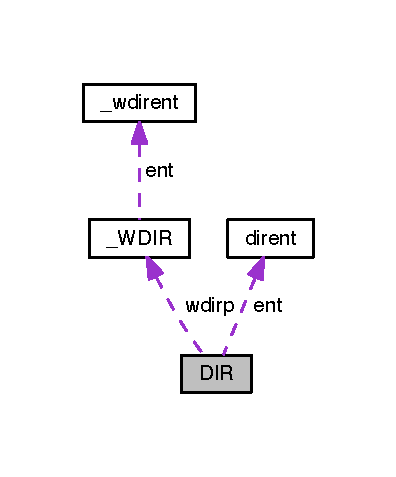
\includegraphics[width=190pt]{struct_d_i_r__coll__graph}
\end{center}
\end{figure}
\subsection*{Public Attributes}
\begin{DoxyCompactItemize}
\item 
struct \hyperlink{structdirent}{dirent} {\bfseries ent}\hypertarget{struct_d_i_r_a59e9f5211cbb2f8e5b2807ccfdd2a7fc}{}\label{struct_d_i_r_a59e9f5211cbb2f8e5b2807ccfdd2a7fc}

\item 
struct \hyperlink{struct___w_d_i_r}{\+\_\+\+W\+D\+IR} $\ast$ {\bfseries wdirp}\hypertarget{struct_d_i_r_a29362d4a3d7f809d0f5418b26cac5d41}{}\label{struct_d_i_r_a29362d4a3d7f809d0f5418b26cac5d41}

\end{DoxyCompactItemize}


The documentation for this struct was generated from the following file\+:\begin{DoxyCompactItemize}
\item 
dirent\+V\+S.\+h\end{DoxyCompactItemize}

\hypertarget{structdirent}{}\section{dirent Struct Reference}
\label{structdirent}\index{dirent@{dirent}}
\subsection*{Public Attributes}
\begin{DoxyCompactItemize}
\item 
long {\bfseries d\+\_\+ino}\hypertarget{structdirent_acb6fecfb0e0f6fdc226dff8d56c3da4a}{}\label{structdirent_acb6fecfb0e0f6fdc226dff8d56c3da4a}

\item 
unsigned short {\bfseries d\+\_\+reclen}\hypertarget{structdirent_a90dc47836e8ef510437317876368859e}{}\label{structdirent_a90dc47836e8ef510437317876368859e}

\item 
size\+\_\+t {\bfseries d\+\_\+namlen}\hypertarget{structdirent_a09ced068b03cdb339e34840c8b709621}{}\label{structdirent_a09ced068b03cdb339e34840c8b709621}

\item 
int {\bfseries d\+\_\+type}\hypertarget{structdirent_ad6a736cb04c7295e8f97f708324b3500}{}\label{structdirent_ad6a736cb04c7295e8f97f708324b3500}

\item 
char {\bfseries d\+\_\+name} \mbox{[}P\+A\+T\+H\+\_\+\+M\+AX\mbox{]}\hypertarget{structdirent_a6c68ac080755453ec52de202e91de59b}{}\label{structdirent_a6c68ac080755453ec52de202e91de59b}

\end{DoxyCompactItemize}


The documentation for this struct was generated from the following file\+:\begin{DoxyCompactItemize}
\item 
dirent\+V\+S.\+h\end{DoxyCompactItemize}

\hypertarget{classviva_1_1_files}{}\section{viva\+:\+:Files Class Reference}
\label{classviva_1_1_files}\index{viva\+::\+Files@{viva\+::\+Files}}


{\ttfamily \#include $<$utils.\+h$>$}

\subsection*{Static Public Member Functions}
\begin{DoxyCompactItemize}
\item 
static string \hyperlink{classviva_1_1_files_a17a0412cc8285a459d0a335bf8835e7f}{tmp\+Filename\+In\+Folder} (const string \&folder=\char`\"{}\char`\"{}, const string \&ext=\char`\"{}.jpg\char`\"{})
\item 
static Rect {\bfseries best\+Square\+From} (Rect \&rectangle)\hypertarget{classviva_1_1_files_aa0d277292b290426118012ffc7e4e0b7}{}\label{classviva_1_1_files_aa0d277292b290426118012ffc7e4e0b7}

\item 
static void {\bfseries save\+Squared\+In} (const Mat \&image, string folder, int side=200)\hypertarget{classviva_1_1_files_a9006758a50b0a9f92a275bf83d2ecc66}{}\label{classviva_1_1_files_a9006758a50b0a9f92a275bf83d2ecc66}

\item 
static void \hyperlink{classviva_1_1_files_a0f1b353d1cad3b64bdcd617a2e0bb356}{listdir} (const string \&dirname, vector$<$ string $>$ \&files, bool return\+Paths=true)
\item 
static void \hyperlink{classviva_1_1_files_a6a1c923fc2fa5ab958ae48d79944cf1d}{list\+Images} (const string \&dirname, vector$<$ string $>$ \&files, bool return\+Paths=true)
\item 
static bool \hyperlink{classviva_1_1_files_ac7835989bfb2b74fb864199362a92e72}{is\+Dir} (const string \&fullpath)
\item 
static bool \hyperlink{classviva_1_1_files_a38538c759fe494f86ac6a310c5409b1a}{is\+File} (const string \&fullpath)
\item 
static void \hyperlink{classviva_1_1_files_a6ffb9c2564fafe3bea2217f0fbccd2d5}{make\+Dir} (const string \&fullpath)
\item 
static bool \hyperlink{classviva_1_1_files_aa65c5d0667235976621e6d51969cdd47}{exists} (const string \&fullpath)
\item 
static void \hyperlink{classviva_1_1_files_ab3c5625f419ae2db28f16c827c53ee42}{get\+Extension} (const string \&filename, string \&extension)
\item 
static void \hyperlink{classviva_1_1_files_abc726ef29d704a2a8c5c75506db76e5b}{get\+Filename} (const string \&path, string \&filename)
\item 
static void \hyperlink{classviva_1_1_files_a0f06aae1db4372c026e5b2d7d7f9647d}{get\+Basename} (const string \&path, string \&base)
\end{DoxyCompactItemize}
\subsection*{Static Public Attributes}
\begin{DoxyCompactItemize}
\item 
static const string {\bfseries P\+A\+T\+H\+\_\+\+S\+E\+P\+A\+R\+A\+T\+OR}
\end{DoxyCompactItemize}


\subsection{Detailed Description}
Set of static functions related to file I/0 operations 

\subsection{Member Function Documentation}
\index{viva\+::\+Files@{viva\+::\+Files}!exists@{exists}}
\index{exists@{exists}!viva\+::\+Files@{viva\+::\+Files}}
\subsubsection[{\texorpdfstring{exists(const string \&fullpath)}{exists(const string &fullpath)}}]{\setlength{\rightskip}{0pt plus 5cm}bool Files\+::exists (
\begin{DoxyParamCaption}
\item[{const string \&}]{fullpath}
\end{DoxyParamCaption}
)\hspace{0.3cm}{\ttfamily [static]}}\hypertarget{classviva_1_1_files_aa65c5d0667235976621e6d51969cdd47}{}\label{classviva_1_1_files_aa65c5d0667235976621e6d51969cdd47}
Checks if the fullpath exits \index{viva\+::\+Files@{viva\+::\+Files}!get\+Basename@{get\+Basename}}
\index{get\+Basename@{get\+Basename}!viva\+::\+Files@{viva\+::\+Files}}
\subsubsection[{\texorpdfstring{get\+Basename(const string \&path, string \&base)}{getBasename(const string &path, string &base)}}]{\setlength{\rightskip}{0pt plus 5cm}void Files\+::get\+Basename (
\begin{DoxyParamCaption}
\item[{const string \&}]{path, }
\item[{string \&}]{base}
\end{DoxyParamCaption}
)\hspace{0.3cm}{\ttfamily [static]}}\hypertarget{classviva_1_1_files_a0f06aae1db4372c026e5b2d7d7f9647d}{}\label{classviva_1_1_files_a0f06aae1db4372c026e5b2d7d7f9647d}
Returns the basename of file in the path \index{viva\+::\+Files@{viva\+::\+Files}!get\+Extension@{get\+Extension}}
\index{get\+Extension@{get\+Extension}!viva\+::\+Files@{viva\+::\+Files}}
\subsubsection[{\texorpdfstring{get\+Extension(const string \&filename, string \&extension)}{getExtension(const string &filename, string &extension)}}]{\setlength{\rightskip}{0pt plus 5cm}void Files\+::get\+Extension (
\begin{DoxyParamCaption}
\item[{const string \&}]{filename, }
\item[{string \&}]{extension}
\end{DoxyParamCaption}
)\hspace{0.3cm}{\ttfamily [static]}}\hypertarget{classviva_1_1_files_ab3c5625f419ae2db28f16c827c53ee42}{}\label{classviva_1_1_files_ab3c5625f419ae2db28f16c827c53ee42}
Returns the extension of the filename \index{viva\+::\+Files@{viva\+::\+Files}!get\+Filename@{get\+Filename}}
\index{get\+Filename@{get\+Filename}!viva\+::\+Files@{viva\+::\+Files}}
\subsubsection[{\texorpdfstring{get\+Filename(const string \&path, string \&filename)}{getFilename(const string &path, string &filename)}}]{\setlength{\rightskip}{0pt plus 5cm}void Files\+::get\+Filename (
\begin{DoxyParamCaption}
\item[{const string \&}]{path, }
\item[{string \&}]{filename}
\end{DoxyParamCaption}
)\hspace{0.3cm}{\ttfamily [static]}}\hypertarget{classviva_1_1_files_abc726ef29d704a2a8c5c75506db76e5b}{}\label{classviva_1_1_files_abc726ef29d704a2a8c5c75506db76e5b}
Returns the filename of file in the path \index{viva\+::\+Files@{viva\+::\+Files}!is\+Dir@{is\+Dir}}
\index{is\+Dir@{is\+Dir}!viva\+::\+Files@{viva\+::\+Files}}
\subsubsection[{\texorpdfstring{is\+Dir(const string \&fullpath)}{isDir(const string &fullpath)}}]{\setlength{\rightskip}{0pt plus 5cm}bool Files\+::is\+Dir (
\begin{DoxyParamCaption}
\item[{const string \&}]{fullpath}
\end{DoxyParamCaption}
)\hspace{0.3cm}{\ttfamily [static]}}\hypertarget{classviva_1_1_files_ac7835989bfb2b74fb864199362a92e72}{}\label{classviva_1_1_files_ac7835989bfb2b74fb864199362a92e72}
Check if path is a directory \index{viva\+::\+Files@{viva\+::\+Files}!is\+File@{is\+File}}
\index{is\+File@{is\+File}!viva\+::\+Files@{viva\+::\+Files}}
\subsubsection[{\texorpdfstring{is\+File(const string \&fullpath)}{isFile(const string &fullpath)}}]{\setlength{\rightskip}{0pt plus 5cm}bool Files\+::is\+File (
\begin{DoxyParamCaption}
\item[{const string \&}]{fullpath}
\end{DoxyParamCaption}
)\hspace{0.3cm}{\ttfamily [static]}}\hypertarget{classviva_1_1_files_a38538c759fe494f86ac6a310c5409b1a}{}\label{classviva_1_1_files_a38538c759fe494f86ac6a310c5409b1a}
Check if path is a regular file \index{viva\+::\+Files@{viva\+::\+Files}!listdir@{listdir}}
\index{listdir@{listdir}!viva\+::\+Files@{viva\+::\+Files}}
\subsubsection[{\texorpdfstring{listdir(const string \&dirname, vector$<$ string $>$ \&files, bool return\+Paths=true)}{listdir(const string &dirname, vector< string > &files, bool returnPaths=true)}}]{\setlength{\rightskip}{0pt plus 5cm}void Files\+::listdir (
\begin{DoxyParamCaption}
\item[{const string \&}]{dirname, }
\item[{vector$<$ string $>$ \&}]{files, }
\item[{bool}]{return\+Paths = {\ttfamily true}}
\end{DoxyParamCaption}
)\hspace{0.3cm}{\ttfamily [static]}}\hypertarget{classviva_1_1_files_a0f1b353d1cad3b64bdcd617a2e0bb356}{}\label{classviva_1_1_files_a0f1b353d1cad3b64bdcd617a2e0bb356}
List directory content and returns it in a vector \index{viva\+::\+Files@{viva\+::\+Files}!list\+Images@{list\+Images}}
\index{list\+Images@{list\+Images}!viva\+::\+Files@{viva\+::\+Files}}
\subsubsection[{\texorpdfstring{list\+Images(const string \&dirname, vector$<$ string $>$ \&files, bool return\+Paths=true)}{listImages(const string &dirname, vector< string > &files, bool returnPaths=true)}}]{\setlength{\rightskip}{0pt plus 5cm}void Files\+::list\+Images (
\begin{DoxyParamCaption}
\item[{const string \&}]{dirname, }
\item[{vector$<$ string $>$ \&}]{files, }
\item[{bool}]{return\+Paths = {\ttfamily true}}
\end{DoxyParamCaption}
)\hspace{0.3cm}{\ttfamily [static]}}\hypertarget{classviva_1_1_files_a6a1c923fc2fa5ab958ae48d79944cf1d}{}\label{classviva_1_1_files_a6a1c923fc2fa5ab958ae48d79944cf1d}
List a directory content and returns a vector of the images contined in it. \index{viva\+::\+Files@{viva\+::\+Files}!make\+Dir@{make\+Dir}}
\index{make\+Dir@{make\+Dir}!viva\+::\+Files@{viva\+::\+Files}}
\subsubsection[{\texorpdfstring{make\+Dir(const string \&fullpath)}{makeDir(const string &fullpath)}}]{\setlength{\rightskip}{0pt plus 5cm}void Files\+::make\+Dir (
\begin{DoxyParamCaption}
\item[{const string \&}]{fullpath}
\end{DoxyParamCaption}
)\hspace{0.3cm}{\ttfamily [static]}}\hypertarget{classviva_1_1_files_a6ffb9c2564fafe3bea2217f0fbccd2d5}{}\label{classviva_1_1_files_a6ffb9c2564fafe3bea2217f0fbccd2d5}
Creates a directory in the specified path \index{viva\+::\+Files@{viva\+::\+Files}!tmp\+Filename\+In\+Folder@{tmp\+Filename\+In\+Folder}}
\index{tmp\+Filename\+In\+Folder@{tmp\+Filename\+In\+Folder}!viva\+::\+Files@{viva\+::\+Files}}
\subsubsection[{\texorpdfstring{tmp\+Filename\+In\+Folder(const string \&folder="""", const string \&ext="".\+jpg"")}{tmpFilenameInFolder(const string &folder="", const string &ext=".jpg")}}]{\setlength{\rightskip}{0pt plus 5cm}string Files\+::tmp\+Filename\+In\+Folder (
\begin{DoxyParamCaption}
\item[{const string \&}]{folder = {\ttfamily \char`\"{}\char`\"{}}, }
\item[{const string \&}]{ext = {\ttfamily \char`\"{}.jpg\char`\"{}}}
\end{DoxyParamCaption}
)\hspace{0.3cm}{\ttfamily [static]}}\hypertarget{classviva_1_1_files_a17a0412cc8285a459d0a335bf8835e7f}{}\label{classviva_1_1_files_a17a0412cc8285a459d0a335bf8835e7f}
Returns a temporary filename inside folder 

\subsection{Member Data Documentation}
\index{viva\+::\+Files@{viva\+::\+Files}!P\+A\+T\+H\+\_\+\+S\+E\+P\+A\+R\+A\+T\+OR@{P\+A\+T\+H\+\_\+\+S\+E\+P\+A\+R\+A\+T\+OR}}
\index{P\+A\+T\+H\+\_\+\+S\+E\+P\+A\+R\+A\+T\+OR@{P\+A\+T\+H\+\_\+\+S\+E\+P\+A\+R\+A\+T\+OR}!viva\+::\+Files@{viva\+::\+Files}}
\subsubsection[{\texorpdfstring{P\+A\+T\+H\+\_\+\+S\+E\+P\+A\+R\+A\+T\+OR}{PATH_SEPARATOR}}]{\setlength{\rightskip}{0pt plus 5cm}const string Files\+::\+P\+A\+T\+H\+\_\+\+S\+E\+P\+A\+R\+A\+T\+OR\hspace{0.3cm}{\ttfamily [static]}}\hypertarget{classviva_1_1_files_a7c2738e3eba6948ce46883dc630f79ee}{}\label{classviva_1_1_files_a7c2738e3eba6948ce46883dc630f79ee}
{\bfseries Initial value\+:}
\begin{DoxyCode}
=



\textcolor{stringliteral}{"/"}
\end{DoxyCode}


The documentation for this class was generated from the following files\+:\begin{DoxyCompactItemize}
\item 
utils.\+h\item 
utils.\+cpp\end{DoxyCompactItemize}

\hypertarget{classviva_1_1_image_list_input}{}\section{viva\+:\+:Image\+List\+Input Class Reference}
\label{classviva_1_1_image_list_input}\index{viva\+::\+Image\+List\+Input@{viva\+::\+Image\+List\+Input}}


{\ttfamily \#include $<$input.\+h$>$}



Inheritance diagram for viva\+:\+:Image\+List\+Input\+:
\nopagebreak
\begin{figure}[H]
\begin{center}
\leavevmode
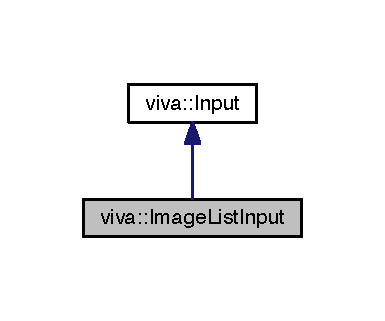
\includegraphics[width=185pt]{classviva_1_1_image_list_input__inherit__graph}
\end{center}
\end{figure}


Collaboration diagram for viva\+:\+:Image\+List\+Input\+:
\nopagebreak
\begin{figure}[H]
\begin{center}
\leavevmode
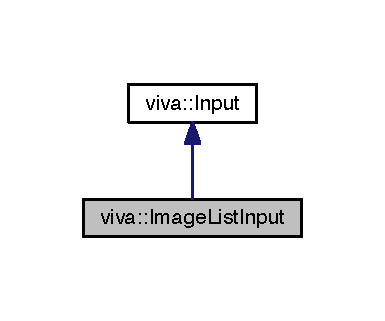
\includegraphics[width=185pt]{classviva_1_1_image_list_input__coll__graph}
\end{center}
\end{figure}
\subsection*{Public Member Functions}
\begin{DoxyCompactItemize}
\item 
\hyperlink{classviva_1_1_image_list_input_aedb635b2155c7e3b99c661c34bd73a4a}{Image\+List\+Input} (const string directory, const Size \&size=Size(-\/1,-\/1), int color\+Flag=-\/1, int loops=1)
\item 
\hyperlink{classviva_1_1_image_list_input_a50fecca0d1f38b8ec70d9da362d72975}{Image\+List\+Input} (const vector$<$ string $>$ \&files, const Size \&size=Size(-\/1,-\/1), int color\+Flag=-\/1, int loops=1)
\item 
bool \hyperlink{classviva_1_1_image_list_input_a0e5759331fb604e55178560de816dbd6}{get\+Frame} (Mat \&frame)
\end{DoxyCompactItemize}
\subsection*{Additional Inherited Members}


\subsection{Detailed Description}
\hyperlink{classviva_1_1_image_list_input}{Image\+List\+Input} to process folder containing images of supported Open\+CV formats. 

\subsection{Constructor \& Destructor Documentation}
\index{viva\+::\+Image\+List\+Input@{viva\+::\+Image\+List\+Input}!Image\+List\+Input@{Image\+List\+Input}}
\index{Image\+List\+Input@{Image\+List\+Input}!viva\+::\+Image\+List\+Input@{viva\+::\+Image\+List\+Input}}
\subsubsection[{\texorpdfstring{Image\+List\+Input(const string directory, const Size \&size=\+Size(-\/1,-\/1), int color\+Flag=-\/1, int loops=1)}{ImageListInput(const string directory, const Size &size=Size(-1,-1), int colorFlag=-1, int loops=1)}}]{\setlength{\rightskip}{0pt plus 5cm}Image\+List\+Input\+::\+Image\+List\+Input (
\begin{DoxyParamCaption}
\item[{const string}]{directory, }
\item[{const Size \&}]{size = {\ttfamily Size(-\/1,-\/1)}, }
\item[{int}]{color\+Flag = {\ttfamily -\/1}, }
\item[{int}]{loops = {\ttfamily 1}}
\end{DoxyParamCaption}
)}\hypertarget{classviva_1_1_image_list_input_aedb635b2155c7e3b99c661c34bd73a4a}{}\label{classviva_1_1_image_list_input_aedb635b2155c7e3b99c661c34bd73a4a}
\hyperlink{classviva_1_1_image_list_input}{Image\+List\+Input} constructor using a directory path \index{viva\+::\+Image\+List\+Input@{viva\+::\+Image\+List\+Input}!Image\+List\+Input@{Image\+List\+Input}}
\index{Image\+List\+Input@{Image\+List\+Input}!viva\+::\+Image\+List\+Input@{viva\+::\+Image\+List\+Input}}
\subsubsection[{\texorpdfstring{Image\+List\+Input(const vector$<$ string $>$ \&files, const Size \&size=\+Size(-\/1,-\/1), int color\+Flag=-\/1, int loops=1)}{ImageListInput(const vector< string > &files, const Size &size=Size(-1,-1), int colorFlag=-1, int loops=1)}}]{\setlength{\rightskip}{0pt plus 5cm}Image\+List\+Input\+::\+Image\+List\+Input (
\begin{DoxyParamCaption}
\item[{const vector$<$ string $>$ \&}]{files, }
\item[{const Size \&}]{size = {\ttfamily Size(-\/1,-\/1)}, }
\item[{int}]{color\+Flag = {\ttfamily -\/1}, }
\item[{int}]{loops = {\ttfamily 1}}
\end{DoxyParamCaption}
)}\hypertarget{classviva_1_1_image_list_input_a50fecca0d1f38b8ec70d9da362d72975}{}\label{classviva_1_1_image_list_input_a50fecca0d1f38b8ec70d9da362d72975}
\hyperlink{classviva_1_1_image_list_input}{Image\+List\+Input} constructor using a vector of filenames containing the images of the sequence in order. 

\subsection{Member Function Documentation}
\index{viva\+::\+Image\+List\+Input@{viva\+::\+Image\+List\+Input}!get\+Frame@{get\+Frame}}
\index{get\+Frame@{get\+Frame}!viva\+::\+Image\+List\+Input@{viva\+::\+Image\+List\+Input}}
\subsubsection[{\texorpdfstring{get\+Frame(\+Mat \&frame)}{getFrame(Mat &frame)}}]{\setlength{\rightskip}{0pt plus 5cm}bool Image\+List\+Input\+::get\+Frame (
\begin{DoxyParamCaption}
\item[{Mat \&}]{frame}
\end{DoxyParamCaption}
)\hspace{0.3cm}{\ttfamily [virtual]}}\hypertarget{classviva_1_1_image_list_input_a0e5759331fb604e55178560de816dbd6}{}\label{classviva_1_1_image_list_input_a0e5759331fb604e55178560de816dbd6}
Overrided from \hyperlink{classviva_1_1_input}{Input} Base Class. Used to extract a frame from the input sequence. Returns whether or not a frame was sucessfuly returned. 
\begin{DoxyParams}{Parameters}
{\em frame} & output image frame from the sequence \\
\hline
\end{DoxyParams}


Implements \hyperlink{classviva_1_1_input_aa24f1c290895fba92d7e1c6032dc4ecb}{viva\+::\+Input}.



The documentation for this class was generated from the following files\+:\begin{DoxyCompactItemize}
\item 
input.\+h\item 
input.\+cpp\end{DoxyCompactItemize}

\hypertarget{classviva_1_1_image_output}{}\section{viva\+:\+:Image\+Output Class Reference}
\label{classviva_1_1_image_output}\index{viva\+::\+Image\+Output@{viva\+::\+Image\+Output}}


{\ttfamily \#include $<$output.\+h$>$}



Inheritance diagram for viva\+:\+:Image\+Output\+:
\nopagebreak
\begin{figure}[H]
\begin{center}
\leavevmode
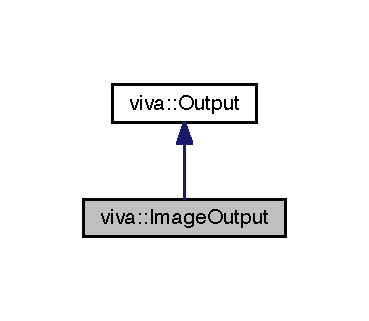
\includegraphics[width=177pt]{classviva_1_1_image_output__inherit__graph}
\end{center}
\end{figure}


Collaboration diagram for viva\+:\+:Image\+Output\+:
\nopagebreak
\begin{figure}[H]
\begin{center}
\leavevmode
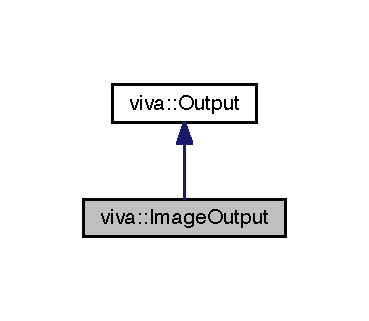
\includegraphics[width=177pt]{classviva_1_1_image_output__coll__graph}
\end{center}
\end{figure}
\subsection*{Public Member Functions}
\begin{DoxyCompactItemize}
\item 
\hyperlink{classviva_1_1_image_output_a157487785ed80da026c0723a3e8aeef5}{Image\+Output} (const string \&directory, const Size \&size=Size(-\/1,-\/1), int suffix\+Size=5, int conversion\+Flag=-\/1)
\item 
virtual bool \hyperlink{classviva_1_1_image_output_a327d64edf5251fe9fb841f348d5b62cb}{write\+Frame} (Mat \&frame)
\end{DoxyCompactItemize}
\subsection*{Additional Inherited Members}


\subsection{Detailed Description}
An Image Sequence \hyperlink{classviva_1_1_output}{Output} that creates a directory an add images using a regular pattern construction filename 

\subsection{Constructor \& Destructor Documentation}
\index{viva\+::\+Image\+Output@{viva\+::\+Image\+Output}!Image\+Output@{Image\+Output}}
\index{Image\+Output@{Image\+Output}!viva\+::\+Image\+Output@{viva\+::\+Image\+Output}}
\subsubsection[{\texorpdfstring{Image\+Output(const string \&directory, const Size \&size=\+Size(-\/1,-\/1), int suffix\+Size=5, int conversion\+Flag=-\/1)}{ImageOutput(const string &directory, const Size &size=Size(-1,-1), int suffixSize=5, int conversionFlag=-1)}}]{\setlength{\rightskip}{0pt plus 5cm}Image\+Output\+::\+Image\+Output (
\begin{DoxyParamCaption}
\item[{const string \&}]{directory, }
\item[{const Size \&}]{size = {\ttfamily Size(-\/1,~-\/1)}, }
\item[{int}]{suffix\+Size = {\ttfamily 5}, }
\item[{int}]{conversion\+Flag = {\ttfamily -\/1}}
\end{DoxyParamCaption}
)}\hypertarget{classviva_1_1_image_output_a157487785ed80da026c0723a3e8aeef5}{}\label{classviva_1_1_image_output_a157487785ed80da026c0723a3e8aeef5}
\hyperlink{classviva_1_1_image_output}{Image\+Output} constructor generates a directory containing a list of images using an incremental regular pattern filename dessign 

\subsection{Member Function Documentation}
\index{viva\+::\+Image\+Output@{viva\+::\+Image\+Output}!write\+Frame@{write\+Frame}}
\index{write\+Frame@{write\+Frame}!viva\+::\+Image\+Output@{viva\+::\+Image\+Output}}
\subsubsection[{\texorpdfstring{write\+Frame(\+Mat \&frame)}{writeFrame(Mat &frame)}}]{\setlength{\rightskip}{0pt plus 5cm}bool Image\+Output\+::write\+Frame (
\begin{DoxyParamCaption}
\item[{Mat \&}]{frame}
\end{DoxyParamCaption}
)\hspace{0.3cm}{\ttfamily [virtual]}}\hypertarget{classviva_1_1_image_output_a327d64edf5251fe9fb841f348d5b62cb}{}\label{classviva_1_1_image_output_a327d64edf5251fe9fb841f348d5b62cb}
Override from \hyperlink{classviva_1_1_output}{Output} Base class 

Implements \hyperlink{classviva_1_1_output_ac74a311b4d151c5507d1351b7fc3426e}{viva\+::\+Output}.



The documentation for this class was generated from the following files\+:\begin{DoxyCompactItemize}
\item 
output.\+h\item 
output.\+cpp\end{DoxyCompactItemize}

\hypertarget{classviva_1_1_input}{}\section{viva\+:\+:Input Class Reference}
\label{classviva_1_1_input}\index{viva\+::\+Input@{viva\+::\+Input}}


{\ttfamily \#include $<$input.\+h$>$}



Inheritance diagram for viva\+:\+:Input\+:
\nopagebreak
\begin{figure}[H]
\begin{center}
\leavevmode
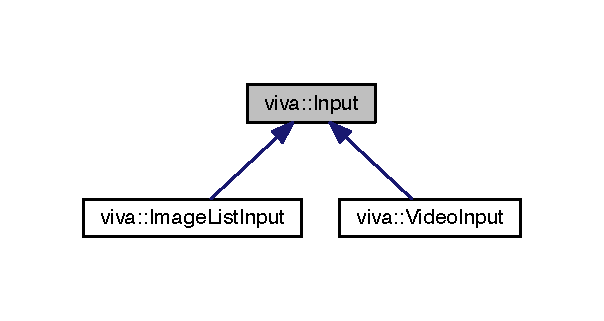
\includegraphics[width=290pt]{classviva_1_1_input__inherit__graph}
\end{center}
\end{figure}
\subsection*{Public Member Functions}
\begin{DoxyCompactItemize}
\item 
\hyperlink{classviva_1_1_input_a4c00744cd1dca9bb025a8b8bc4c9541d}{Input} (const Size \&size=Size(-\/1,-\/1), int conversion\+Flag=-\/1)
\item 
virtual bool \hyperlink{classviva_1_1_input_aa24f1c290895fba92d7e1c6032dc4ecb}{get\+Frame} (Mat \&image)=0
\item 
virtual \hyperlink{classviva_1_1_input_a278d491b01b3e2b76683b8949549250b}{$\sim$\+Input} ()
\item 
void \hyperlink{classviva_1_1_input_a9b0fbd57dd4c1c68428174530c588694}{set\+Conversion\+Type} (int flag)
\item 
size\+\_\+t \hyperlink{classviva_1_1_input_a510a003dcbd21eef8a10912d648293c7}{get\+Width} ()
\item 
size\+\_\+t \hyperlink{classviva_1_1_input_adebf24bbf1bd6306fcd7f0ff38149a43}{get\+Height} ()
\item 
Size \hyperlink{classviva_1_1_input_a0c7faa4c9daf1e46caf7d80994ea4ef5}{get\+Org\+Size} ()
\end{DoxyCompactItemize}
\subsection*{Protected Attributes}
\begin{DoxyCompactItemize}
\item 
Size {\bfseries \+\_\+size}\hypertarget{classviva_1_1_input_a987798abae2d1a624452bc78e1bfc697}{}\label{classviva_1_1_input_a987798abae2d1a624452bc78e1bfc697}

\item 
bool {\bfseries \+\_\+convert}\hypertarget{classviva_1_1_input_a70d7f2d92f128ee2381edb7acd39266f}{}\label{classviva_1_1_input_a70d7f2d92f128ee2381edb7acd39266f}

\item 
int {\bfseries \+\_\+conversion\+Flag}\hypertarget{classviva_1_1_input_ab86c4dc7244fc837b26fe53dd07b4a9b}{}\label{classviva_1_1_input_ab86c4dc7244fc837b26fe53dd07b4a9b}

\item 
Size {\bfseries \+\_\+org\+Size}\hypertarget{classviva_1_1_input_ad70fb7270e0c587f2376b1a7ec9c35fc}{}\label{classviva_1_1_input_ad70fb7270e0c587f2376b1a7ec9c35fc}

\end{DoxyCompactItemize}


\subsection{Detailed Description}
Abstract \hyperlink{classviva_1_1_input}{Input} Class defining the interface for a video sequence input type. 

\subsection{Constructor \& Destructor Documentation}
\index{viva\+::\+Input@{viva\+::\+Input}!Input@{Input}}
\index{Input@{Input}!viva\+::\+Input@{viva\+::\+Input}}
\subsubsection[{\texorpdfstring{Input(const Size \&size=\+Size(-\/1,-\/1), int conversion\+Flag=-\/1)}{Input(const Size &size=Size(-1,-1), int conversionFlag=-1)}}]{\setlength{\rightskip}{0pt plus 5cm}viva\+::\+Input\+::\+Input (
\begin{DoxyParamCaption}
\item[{const Size \&}]{size = {\ttfamily Size(-\/1,~-\/1)}, }
\item[{int}]{conversion\+Flag = {\ttfamily -\/1}}
\end{DoxyParamCaption}
)\hspace{0.3cm}{\ttfamily [inline]}}\hypertarget{classviva_1_1_input_a4c00744cd1dca9bb025a8b8bc4c9541d}{}\label{classviva_1_1_input_a4c00744cd1dca9bb025a8b8bc4c9541d}
\hyperlink{classviva_1_1_input}{Input} class constructor 
\begin{DoxyParams}{Parameters}
{\em size} & force the input class to an specific size resolution. Default value of (-\/1,-\/1) will use the original medium resolution. \\
\hline
{\em conversion\+Flag} & Open\+CV conversion flag e.\+g., C\+V\+\_\+\+R\+G\+B2\+G\+R\+AY. Default value of -\/1 will do not convert the original feed. \\
\hline
\end{DoxyParams}
\index{viva\+::\+Input@{viva\+::\+Input}!````~Input@{$\sim$\+Input}}
\index{````~Input@{$\sim$\+Input}!viva\+::\+Input@{viva\+::\+Input}}
\subsubsection[{\texorpdfstring{$\sim$\+Input()}{~Input()}}]{\setlength{\rightskip}{0pt plus 5cm}virtual viva\+::\+Input\+::$\sim$\+Input (
\begin{DoxyParamCaption}
{}
\end{DoxyParamCaption}
)\hspace{0.3cm}{\ttfamily [inline]}, {\ttfamily [virtual]}}\hypertarget{classviva_1_1_input_a278d491b01b3e2b76683b8949549250b}{}\label{classviva_1_1_input_a278d491b01b3e2b76683b8949549250b}
Virtual desctructor 

\subsection{Member Function Documentation}
\index{viva\+::\+Input@{viva\+::\+Input}!get\+Frame@{get\+Frame}}
\index{get\+Frame@{get\+Frame}!viva\+::\+Input@{viva\+::\+Input}}
\subsubsection[{\texorpdfstring{get\+Frame(\+Mat \&image)=0}{getFrame(Mat &image)=0}}]{\setlength{\rightskip}{0pt plus 5cm}virtual bool viva\+::\+Input\+::get\+Frame (
\begin{DoxyParamCaption}
\item[{Mat \&}]{image}
\end{DoxyParamCaption}
)\hspace{0.3cm}{\ttfamily [pure virtual]}}\hypertarget{classviva_1_1_input_aa24f1c290895fba92d7e1c6032dc4ecb}{}\label{classviva_1_1_input_aa24f1c290895fba92d7e1c6032dc4ecb}
Obtain an image frame from the input 
\begin{DoxyParams}{Parameters}
{\em image} & output image from the input. \\
\hline
\end{DoxyParams}
\begin{DoxyReturn}{Returns}
bool\+: whenever an image was retrieved or not from the input. 
\end{DoxyReturn}


Implemented in \hyperlink{classviva_1_1_image_list_input_a0e5759331fb604e55178560de816dbd6}{viva\+::\+Image\+List\+Input}, and \hyperlink{classviva_1_1_video_input_ab4819eb95ad41ba9a59536f60eefa5a9}{viva\+::\+Video\+Input}.

\index{viva\+::\+Input@{viva\+::\+Input}!get\+Height@{get\+Height}}
\index{get\+Height@{get\+Height}!viva\+::\+Input@{viva\+::\+Input}}
\subsubsection[{\texorpdfstring{get\+Height()}{getHeight()}}]{\setlength{\rightskip}{0pt plus 5cm}size\+\_\+t viva\+::\+Input\+::get\+Height (
\begin{DoxyParamCaption}
{}
\end{DoxyParamCaption}
)\hspace{0.3cm}{\ttfamily [inline]}}\hypertarget{classviva_1_1_input_adebf24bbf1bd6306fcd7f0ff38149a43}{}\label{classviva_1_1_input_adebf24bbf1bd6306fcd7f0ff38149a43}
Returns the image\textquotesingle{}s height of the input feed \index{viva\+::\+Input@{viva\+::\+Input}!get\+Org\+Size@{get\+Org\+Size}}
\index{get\+Org\+Size@{get\+Org\+Size}!viva\+::\+Input@{viva\+::\+Input}}
\subsubsection[{\texorpdfstring{get\+Org\+Size()}{getOrgSize()}}]{\setlength{\rightskip}{0pt plus 5cm}Size viva\+::\+Input\+::get\+Org\+Size (
\begin{DoxyParamCaption}
{}
\end{DoxyParamCaption}
)\hspace{0.3cm}{\ttfamily [inline]}}\hypertarget{classviva_1_1_input_a0c7faa4c9daf1e46caf7d80994ea4ef5}{}\label{classviva_1_1_input_a0c7faa4c9daf1e46caf7d80994ea4ef5}
Returns the original input size. This will be the same to the current image\textquotesingle{}s width and height if it\textquotesingle{}s created with size(-\/1,-\/1). \index{viva\+::\+Input@{viva\+::\+Input}!get\+Width@{get\+Width}}
\index{get\+Width@{get\+Width}!viva\+::\+Input@{viva\+::\+Input}}
\subsubsection[{\texorpdfstring{get\+Width()}{getWidth()}}]{\setlength{\rightskip}{0pt plus 5cm}size\+\_\+t viva\+::\+Input\+::get\+Width (
\begin{DoxyParamCaption}
{}
\end{DoxyParamCaption}
)\hspace{0.3cm}{\ttfamily [inline]}}\hypertarget{classviva_1_1_input_a510a003dcbd21eef8a10912d648293c7}{}\label{classviva_1_1_input_a510a003dcbd21eef8a10912d648293c7}
Returns the image\textquotesingle{}s width of the input feed. \index{viva\+::\+Input@{viva\+::\+Input}!set\+Conversion\+Type@{set\+Conversion\+Type}}
\index{set\+Conversion\+Type@{set\+Conversion\+Type}!viva\+::\+Input@{viva\+::\+Input}}
\subsubsection[{\texorpdfstring{set\+Conversion\+Type(int flag)}{setConversionType(int flag)}}]{\setlength{\rightskip}{0pt plus 5cm}void viva\+::\+Input\+::set\+Conversion\+Type (
\begin{DoxyParamCaption}
\item[{int}]{flag}
\end{DoxyParamCaption}
)\hspace{0.3cm}{\ttfamily [inline]}}\hypertarget{classviva_1_1_input_a9b0fbd57dd4c1c68428174530c588694}{}\label{classviva_1_1_input_a9b0fbd57dd4c1c68428174530c588694}
Set the Open\+CV conversion flag value e.\+g., C\+V\+\_\+\+B\+G\+R2\+G\+R\+AY. Any posterior call to process\+Frame will return an image using this conversion type flag. 

The documentation for this class was generated from the following file\+:\begin{DoxyCompactItemize}
\item 
input.\+h\end{DoxyCompactItemize}

\hypertarget{classviva_1_1_keyboard_listener}{}\section{viva\+:\+:Keyboard\+Listener Class Reference}
\label{classviva_1_1_keyboard_listener}\index{viva\+::\+Keyboard\+Listener@{viva\+::\+Keyboard\+Listener}}


{\ttfamily \#include $<$listener.\+h$>$}



Inheritance diagram for viva\+:\+:Keyboard\+Listener\+:
\nopagebreak
\begin{figure}[H]
\begin{center}
\leavevmode
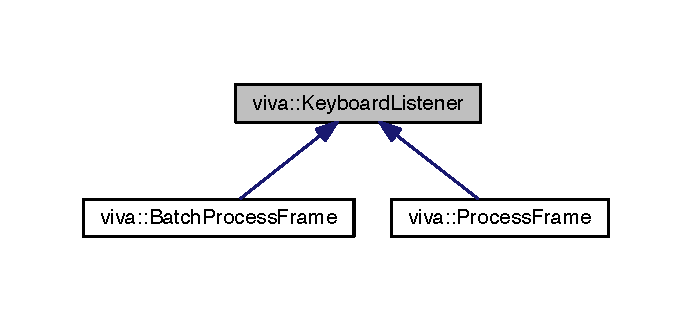
\includegraphics[width=332pt]{classviva_1_1_keyboard_listener__inherit__graph}
\end{center}
\end{figure}
\subsection*{Public Member Functions}
\begin{DoxyCompactItemize}
\item 
virtual void \hyperlink{classviva_1_1_keyboard_listener_a903947e765f8130cfe1b3ce882c95998}{keyboard\+Input} (int key)
\end{DoxyCompactItemize}


\subsection{Detailed Description}
\hyperlink{classviva_1_1_keyboard_listener}{Keyboard\+Listener} interface 

\subsection{Member Function Documentation}
\index{viva\+::\+Keyboard\+Listener@{viva\+::\+Keyboard\+Listener}!keyboard\+Input@{keyboard\+Input}}
\index{keyboard\+Input@{keyboard\+Input}!viva\+::\+Keyboard\+Listener@{viva\+::\+Keyboard\+Listener}}
\subsubsection[{\texorpdfstring{keyboard\+Input(int key)}{keyboardInput(int key)}}]{\setlength{\rightskip}{0pt plus 5cm}virtual void viva\+::\+Keyboard\+Listener\+::keyboard\+Input (
\begin{DoxyParamCaption}
\item[{int}]{key}
\end{DoxyParamCaption}
)\hspace{0.3cm}{\ttfamily [inline]}, {\ttfamily [virtual]}}\hypertarget{classviva_1_1_keyboard_listener_a903947e765f8130cfe1b3ce882c95998}{}\label{classviva_1_1_keyboard_listener_a903947e765f8130cfe1b3ce882c95998}
It will be called only when the user stroke a keyboard key 
\begin{DoxyParams}{Parameters}
{\em key} & the value of the pressed key \\
\hline
\end{DoxyParams}


Reimplemented in \hyperlink{classviva_1_1_batch_process_frame_a956265d099d3b4f4305045bfccceb308}{viva\+::\+Batch\+Process\+Frame}, and \hyperlink{classviva_1_1_process_frame_a56d6805a983de9072ce31ea60688a408}{viva\+::\+Process\+Frame}.



The documentation for this class was generated from the following file\+:\begin{DoxyCompactItemize}
\item 
listener.\+h\end{DoxyCompactItemize}

\hypertarget{structviva_1_1_keys}{}\section{viva\+:\+:Keys Struct Reference}
\label{structviva_1_1_keys}\index{viva\+::\+Keys@{viva\+::\+Keys}}


{\ttfamily \#include $<$utils.\+h$>$}

\subsection*{Static Public Attributes}
\begin{DoxyCompactItemize}
\item 
static const int {\bfseries E\+SC} = 27\hypertarget{structviva_1_1_keys_ac6523bc0746965636ffdc68d3f436a23}{}\label{structviva_1_1_keys_ac6523bc0746965636ffdc68d3f436a23}

\item 
static const int {\bfseries T\+AB} = 9\hypertarget{structviva_1_1_keys_a6e7ea2431a204ae4bf423e991304b560}{}\label{structviva_1_1_keys_a6e7ea2431a204ae4bf423e991304b560}

\item 
static const int {\bfseries S\+P\+A\+CE} = 32\hypertarget{structviva_1_1_keys_a002c97e8fff639c0fd8b6aa26bc89d35}{}\label{structviva_1_1_keys_a002c97e8fff639c0fd8b6aa26bc89d35}

\item 
static const int {\bfseries N\+O\+NE} = -\/1\hypertarget{structviva_1_1_keys_a28978a62c674741157417b5261eb7984}{}\label{structviva_1_1_keys_a28978a62c674741157417b5261eb7984}

\item 
static const int {\bfseries c} = \textquotesingle{}c\textquotesingle{}\hypertarget{structviva_1_1_keys_a54cb8ed20e50156e2ca257163ccf97de}{}\label{structviva_1_1_keys_a54cb8ed20e50156e2ca257163ccf97de}

\end{DoxyCompactItemize}


\subsection{Detailed Description}
Set of custom keys used in the G\+UI. The E\+SC key will exit the applicaiton The S\+P\+A\+CE will pause and resume the video sequence 

The documentation for this struct was generated from the following files\+:\begin{DoxyCompactItemize}
\item 
utils.\+h\item 
utils.\+cpp\end{DoxyCompactItemize}

\hypertarget{classviva_1_1_mouse_listener}{}\section{viva\+:\+:Mouse\+Listener Class Reference}
\label{classviva_1_1_mouse_listener}\index{viva\+::\+Mouse\+Listener@{viva\+::\+Mouse\+Listener}}


{\ttfamily \#include $<$listener.\+h$>$}



Inheritance diagram for viva\+:\+:Mouse\+Listener\+:
\nopagebreak
\begin{figure}[H]
\begin{center}
\leavevmode
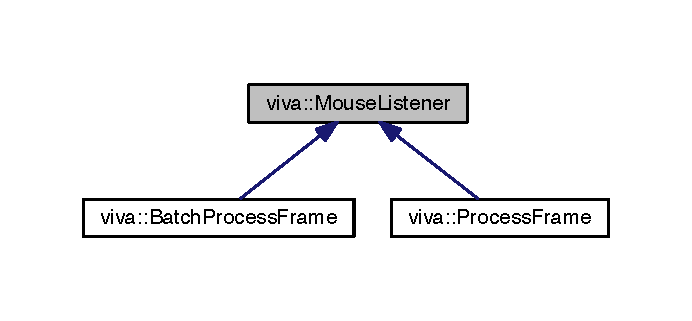
\includegraphics[width=332pt]{classviva_1_1_mouse_listener__inherit__graph}
\end{center}
\end{figure}
\subsection*{Public Member Functions}
\begin{DoxyCompactItemize}
\item 
virtual void \hyperlink{classviva_1_1_mouse_listener_aba95f99370a82ae96f89fe9a1eebd00b}{mouse\+Input} (int event, int x, int y, int flags)
\item 
virtual void \hyperlink{classviva_1_1_mouse_listener_ae2b6952da67ea99e47f5fcfa2e1780c7}{left\+Button\+Down} (int x, int y, int flags)
\item 
virtual void \hyperlink{classviva_1_1_mouse_listener_ae4a2d181ecebf2e4001ce6440339ed60}{right\+Button\+Down} (int x, int y, int flags)
\item 
virtual void \hyperlink{classviva_1_1_mouse_listener_a3a61b77b23875e74f817020ee1603556}{middle\+Button\+Down} (int x, int y, int flags)
\item 
virtual void \hyperlink{classviva_1_1_mouse_listener_af48bb769c4935f52646567118cb05900}{mouse\+Move} (int x, int y, int flags)
\end{DoxyCompactItemize}


\subsection{Detailed Description}
\hyperlink{classviva_1_1_mouse_listener}{Mouse\+Listener} Interface 

\subsection{Member Function Documentation}
\index{viva\+::\+Mouse\+Listener@{viva\+::\+Mouse\+Listener}!left\+Button\+Down@{left\+Button\+Down}}
\index{left\+Button\+Down@{left\+Button\+Down}!viva\+::\+Mouse\+Listener@{viva\+::\+Mouse\+Listener}}
\subsubsection[{\texorpdfstring{left\+Button\+Down(int x, int y, int flags)}{leftButtonDown(int x, int y, int flags)}}]{\setlength{\rightskip}{0pt plus 5cm}virtual void viva\+::\+Mouse\+Listener\+::left\+Button\+Down (
\begin{DoxyParamCaption}
\item[{int}]{x, }
\item[{int}]{y, }
\item[{int}]{flags}
\end{DoxyParamCaption}
)\hspace{0.3cm}{\ttfamily [inline]}, {\ttfamily [virtual]}}\hypertarget{classviva_1_1_mouse_listener_ae2b6952da67ea99e47f5fcfa2e1780c7}{}\label{classviva_1_1_mouse_listener_ae2b6952da67ea99e47f5fcfa2e1780c7}
It will be called only when a mouse left click is triggered 

Reimplemented in \hyperlink{classviva_1_1_batch_process_frame_a7b4b1dbd173e0d900e7d1461c373fdad}{viva\+::\+Batch\+Process\+Frame}, and \hyperlink{classviva_1_1_process_frame_a1d0476b4a6065fae4c0b46abf230be1c}{viva\+::\+Process\+Frame}.

\index{viva\+::\+Mouse\+Listener@{viva\+::\+Mouse\+Listener}!middle\+Button\+Down@{middle\+Button\+Down}}
\index{middle\+Button\+Down@{middle\+Button\+Down}!viva\+::\+Mouse\+Listener@{viva\+::\+Mouse\+Listener}}
\subsubsection[{\texorpdfstring{middle\+Button\+Down(int x, int y, int flags)}{middleButtonDown(int x, int y, int flags)}}]{\setlength{\rightskip}{0pt plus 5cm}virtual void viva\+::\+Mouse\+Listener\+::middle\+Button\+Down (
\begin{DoxyParamCaption}
\item[{int}]{x, }
\item[{int}]{y, }
\item[{int}]{flags}
\end{DoxyParamCaption}
)\hspace{0.3cm}{\ttfamily [inline]}, {\ttfamily [virtual]}}\hypertarget{classviva_1_1_mouse_listener_a3a61b77b23875e74f817020ee1603556}{}\label{classviva_1_1_mouse_listener_a3a61b77b23875e74f817020ee1603556}
It will be called only when a mouse middle click is triggered 

Reimplemented in \hyperlink{classviva_1_1_batch_process_frame_a34fc0aff605d24a0260f466cd386c091}{viva\+::\+Batch\+Process\+Frame}, and \hyperlink{classviva_1_1_process_frame_a2c5155855fa6a88bb8124278ece845ee}{viva\+::\+Process\+Frame}.

\index{viva\+::\+Mouse\+Listener@{viva\+::\+Mouse\+Listener}!mouse\+Input@{mouse\+Input}}
\index{mouse\+Input@{mouse\+Input}!viva\+::\+Mouse\+Listener@{viva\+::\+Mouse\+Listener}}
\subsubsection[{\texorpdfstring{mouse\+Input(int event, int x, int y, int flags)}{mouseInput(int event, int x, int y, int flags)}}]{\setlength{\rightskip}{0pt plus 5cm}virtual void viva\+::\+Mouse\+Listener\+::mouse\+Input (
\begin{DoxyParamCaption}
\item[{int}]{event, }
\item[{int}]{x, }
\item[{int}]{y, }
\item[{int}]{flags}
\end{DoxyParamCaption}
)\hspace{0.3cm}{\ttfamily [inline]}, {\ttfamily [virtual]}}\hypertarget{classviva_1_1_mouse_listener_aba95f99370a82ae96f89fe9a1eebd00b}{}\label{classviva_1_1_mouse_listener_aba95f99370a82ae96f89fe9a1eebd00b}
Will be triggered at any mouse event, the type of the event is especified in the first integer 
\begin{DoxyParams}{Parameters}
{\em event.} & event could be one of the following Open\+CV values E\+V\+E\+N\+T\+\_\+\+L\+B\+U\+T\+T\+O\+N\+D\+O\+WN, E\+V\+E\+N\+T\+\_\+\+R\+B\+U\+T\+T\+O\+N\+D\+O\+WN, E\+V\+E\+N\+T\+\_\+\+M\+B\+U\+T\+T\+O\+N\+D\+O\+WN, E\+V\+E\+N\+T\+\_\+\+M\+O\+U\+S\+E\+M\+O\+VE. \\
\hline
{\em x} & the x coordinates of the mouse cursor \\
\hline
{\em y} & the y coordinates of the mouse cursor \\
\hline
{\em flgas} & the flags passed from Open\+CV \\
\hline
\end{DoxyParams}


Reimplemented in \hyperlink{classviva_1_1_batch_process_frame_a70b9f91a0d9fadb04ec4db3df7fbd2a8}{viva\+::\+Batch\+Process\+Frame}, and \hyperlink{classviva_1_1_process_frame_a67f1444128085a4f18b6c7fe5086e6fc}{viva\+::\+Process\+Frame}.

\index{viva\+::\+Mouse\+Listener@{viva\+::\+Mouse\+Listener}!mouse\+Move@{mouse\+Move}}
\index{mouse\+Move@{mouse\+Move}!viva\+::\+Mouse\+Listener@{viva\+::\+Mouse\+Listener}}
\subsubsection[{\texorpdfstring{mouse\+Move(int x, int y, int flags)}{mouseMove(int x, int y, int flags)}}]{\setlength{\rightskip}{0pt plus 5cm}virtual void viva\+::\+Mouse\+Listener\+::mouse\+Move (
\begin{DoxyParamCaption}
\item[{int}]{x, }
\item[{int}]{y, }
\item[{int}]{flags}
\end{DoxyParamCaption}
)\hspace{0.3cm}{\ttfamily [inline]}, {\ttfamily [virtual]}}\hypertarget{classviva_1_1_mouse_listener_af48bb769c4935f52646567118cb05900}{}\label{classviva_1_1_mouse_listener_af48bb769c4935f52646567118cb05900}
It will be called only when a mouse move is triggered. 

Reimplemented in \hyperlink{classviva_1_1_batch_process_frame_afaf81db14d5a7f6f97c766498c9b66c9}{viva\+::\+Batch\+Process\+Frame}, and \hyperlink{classviva_1_1_process_frame_a075654580641032ff792eedd3fd6b7a1}{viva\+::\+Process\+Frame}.

\index{viva\+::\+Mouse\+Listener@{viva\+::\+Mouse\+Listener}!right\+Button\+Down@{right\+Button\+Down}}
\index{right\+Button\+Down@{right\+Button\+Down}!viva\+::\+Mouse\+Listener@{viva\+::\+Mouse\+Listener}}
\subsubsection[{\texorpdfstring{right\+Button\+Down(int x, int y, int flags)}{rightButtonDown(int x, int y, int flags)}}]{\setlength{\rightskip}{0pt plus 5cm}virtual void viva\+::\+Mouse\+Listener\+::right\+Button\+Down (
\begin{DoxyParamCaption}
\item[{int}]{x, }
\item[{int}]{y, }
\item[{int}]{flags}
\end{DoxyParamCaption}
)\hspace{0.3cm}{\ttfamily [inline]}, {\ttfamily [virtual]}}\hypertarget{classviva_1_1_mouse_listener_ae4a2d181ecebf2e4001ce6440339ed60}{}\label{classviva_1_1_mouse_listener_ae4a2d181ecebf2e4001ce6440339ed60}
It will be called only when a right left click is triggered 

Reimplemented in \hyperlink{classviva_1_1_batch_process_frame_ab7b8be0c726713cbf8be004ed9974ec6}{viva\+::\+Batch\+Process\+Frame}, and \hyperlink{classviva_1_1_process_frame_a03b8c90d990dcefdddf4ad735290d0eb}{viva\+::\+Process\+Frame}.



The documentation for this class was generated from the following file\+:\begin{DoxyCompactItemize}
\item 
listener.\+h\end{DoxyCompactItemize}

\hypertarget{classviva_1_1_none_output}{}\section{viva\+:\+:None\+Output Class Reference}
\label{classviva_1_1_none_output}\index{viva\+::\+None\+Output@{viva\+::\+None\+Output}}


{\ttfamily \#include $<$output.\+h$>$}



Inheritance diagram for viva\+:\+:None\+Output\+:
\nopagebreak
\begin{figure}[H]
\begin{center}
\leavevmode
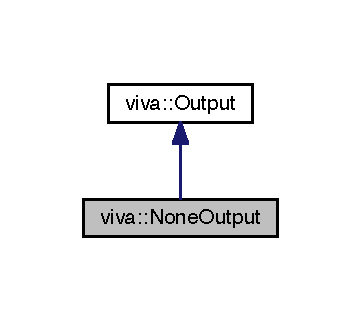
\includegraphics[width=173pt]{classviva_1_1_none_output__inherit__graph}
\end{center}
\end{figure}


Collaboration diagram for viva\+:\+:None\+Output\+:
\nopagebreak
\begin{figure}[H]
\begin{center}
\leavevmode
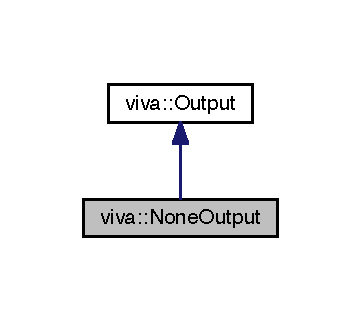
\includegraphics[width=173pt]{classviva_1_1_none_output__coll__graph}
\end{center}
\end{figure}
\subsection*{Public Member Functions}
\begin{DoxyCompactItemize}
\item 
{\bfseries None\+Output} (const Size \&size=Size(-\/1,-\/1), int color\+Flag=-\/1)\hypertarget{classviva_1_1_none_output_a71f975278ec4ebc414a9e135ce307bb0}{}\label{classviva_1_1_none_output_a71f975278ec4ebc414a9e135ce307bb0}

\item 
bool \hyperlink{classviva_1_1_none_output_a0f00d1d9c6ca1af279fd566044ef7f60}{write\+Frame} (Mat \&frame)
\end{DoxyCompactItemize}
\subsection*{Additional Inherited Members}


\subsection{Detailed Description}
An \hyperlink{classviva_1_1_output}{Output} class that does nothing. 

\subsection{Member Function Documentation}
\index{viva\+::\+None\+Output@{viva\+::\+None\+Output}!write\+Frame@{write\+Frame}}
\index{write\+Frame@{write\+Frame}!viva\+::\+None\+Output@{viva\+::\+None\+Output}}
\subsubsection[{\texorpdfstring{write\+Frame(\+Mat \&frame)}{writeFrame(Mat &frame)}}]{\setlength{\rightskip}{0pt plus 5cm}bool viva\+::\+None\+Output\+::write\+Frame (
\begin{DoxyParamCaption}
\item[{Mat \&}]{frame}
\end{DoxyParamCaption}
)\hspace{0.3cm}{\ttfamily [inline]}, {\ttfamily [virtual]}}\hypertarget{classviva_1_1_none_output_a0f00d1d9c6ca1af279fd566044ef7f60}{}\label{classviva_1_1_none_output_a0f00d1d9c6ca1af279fd566044ef7f60}
Method call to output a new frame to the final output sequence \begin{DoxyReturn}{Returns}
true if the Mat frame was sucessfully written 
\end{DoxyReturn}


Implements \hyperlink{classviva_1_1_output_ac74a311b4d151c5507d1351b7fc3426e}{viva\+::\+Output}.



The documentation for this class was generated from the following file\+:\begin{DoxyCompactItemize}
\item 
output.\+h\end{DoxyCompactItemize}

\hypertarget{classviva_1_1_output}{}\section{viva\+:\+:Output Class Reference}
\label{classviva_1_1_output}\index{viva\+::\+Output@{viva\+::\+Output}}


{\ttfamily \#include $<$output.\+h$>$}



Inheritance diagram for viva\+:\+:Output\+:
\nopagebreak
\begin{figure}[H]
\begin{center}
\leavevmode
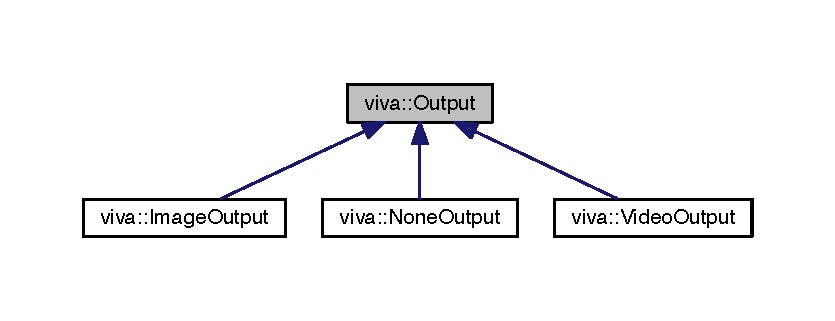
\includegraphics[width=350pt]{classviva_1_1_output__inherit__graph}
\end{center}
\end{figure}
\subsection*{Public Member Functions}
\begin{DoxyCompactItemize}
\item 
\hyperlink{classviva_1_1_output_a184b70bb8e871a6e538e5dae1794de9a}{Output} (const Size \&size=Size(-\/1,-\/1), int conversion\+Flag=-\/1)
\item 
virtual \hyperlink{classviva_1_1_output_a54e4b6572be4e5c2affde8eead501a5d}{$\sim$\+Output} ()
\item 
virtual bool \hyperlink{classviva_1_1_output_ac74a311b4d151c5507d1351b7fc3426e}{write\+Frame} (Mat \&frame)=0
\item 
virtual void \hyperlink{classviva_1_1_output_a6fc610f298473208bf780ccec88dd018}{close} ()
\end{DoxyCompactItemize}
\subsection*{Protected Attributes}
\begin{DoxyCompactItemize}
\item 
Size {\bfseries \+\_\+size}\hypertarget{classviva_1_1_output_a8f7f08a43c3c7381420541faf65e940c}{}\label{classviva_1_1_output_a8f7f08a43c3c7381420541faf65e940c}

\item 
bool {\bfseries \+\_\+convert}\hypertarget{classviva_1_1_output_ac60b23056f3df565dec684751c3ada23}{}\label{classviva_1_1_output_ac60b23056f3df565dec684751c3ada23}

\item 
int {\bfseries \+\_\+conversion\+Flag}\hypertarget{classviva_1_1_output_ad65736a928c2aa6613276b6ee2ee8045}{}\label{classviva_1_1_output_ad65736a928c2aa6613276b6ee2ee8045}

\end{DoxyCompactItemize}


\subsection{Detailed Description}
Abstract \hyperlink{classviva_1_1_output}{Output} class to define a video sequence output. 

\subsection{Constructor \& Destructor Documentation}
\index{viva\+::\+Output@{viva\+::\+Output}!Output@{Output}}
\index{Output@{Output}!viva\+::\+Output@{viva\+::\+Output}}
\subsubsection[{\texorpdfstring{Output(const Size \&size=\+Size(-\/1,-\/1), int conversion\+Flag=-\/1)}{Output(const Size &size=Size(-1,-1), int conversionFlag=-1)}}]{\setlength{\rightskip}{0pt plus 5cm}viva\+::\+Output\+::\+Output (
\begin{DoxyParamCaption}
\item[{const Size \&}]{size = {\ttfamily Size(-\/1,~-\/1)}, }
\item[{int}]{conversion\+Flag = {\ttfamily -\/1}}
\end{DoxyParamCaption}
)\hspace{0.3cm}{\ttfamily [inline]}}\hypertarget{classviva_1_1_output_a184b70bb8e871a6e538e5dae1794de9a}{}\label{classviva_1_1_output_a184b70bb8e871a6e538e5dae1794de9a}
\hyperlink{classviva_1_1_output}{Output} constructor defining the resolution and video type using Open\+CV conversion flags e.\+g., C\+V\+\_\+\+B\+G\+R2\+G\+R\+AY \index{viva\+::\+Output@{viva\+::\+Output}!````~Output@{$\sim$\+Output}}
\index{````~Output@{$\sim$\+Output}!viva\+::\+Output@{viva\+::\+Output}}
\subsubsection[{\texorpdfstring{$\sim$\+Output()}{~Output()}}]{\setlength{\rightskip}{0pt plus 5cm}virtual viva\+::\+Output\+::$\sim$\+Output (
\begin{DoxyParamCaption}
{}
\end{DoxyParamCaption}
)\hspace{0.3cm}{\ttfamily [inline]}, {\ttfamily [virtual]}}\hypertarget{classviva_1_1_output_a54e4b6572be4e5c2affde8eead501a5d}{}\label{classviva_1_1_output_a54e4b6572be4e5c2affde8eead501a5d}
Desctructor 

\subsection{Member Function Documentation}
\index{viva\+::\+Output@{viva\+::\+Output}!close@{close}}
\index{close@{close}!viva\+::\+Output@{viva\+::\+Output}}
\subsubsection[{\texorpdfstring{close()}{close()}}]{\setlength{\rightskip}{0pt plus 5cm}virtual void viva\+::\+Output\+::close (
\begin{DoxyParamCaption}
{}
\end{DoxyParamCaption}
)\hspace{0.3cm}{\ttfamily [inline]}, {\ttfamily [virtual]}}\hypertarget{classviva_1_1_output_a6fc610f298473208bf780ccec88dd018}{}\label{classviva_1_1_output_a6fc610f298473208bf780ccec88dd018}
Mehtod called to close the output medium \index{viva\+::\+Output@{viva\+::\+Output}!write\+Frame@{write\+Frame}}
\index{write\+Frame@{write\+Frame}!viva\+::\+Output@{viva\+::\+Output}}
\subsubsection[{\texorpdfstring{write\+Frame(\+Mat \&frame)=0}{writeFrame(Mat &frame)=0}}]{\setlength{\rightskip}{0pt plus 5cm}virtual bool viva\+::\+Output\+::write\+Frame (
\begin{DoxyParamCaption}
\item[{Mat \&}]{frame}
\end{DoxyParamCaption}
)\hspace{0.3cm}{\ttfamily [pure virtual]}}\hypertarget{classviva_1_1_output_ac74a311b4d151c5507d1351b7fc3426e}{}\label{classviva_1_1_output_ac74a311b4d151c5507d1351b7fc3426e}
Method call to output a new frame to the final output sequence \begin{DoxyReturn}{Returns}
true if the Mat frame was sucessfully written 
\end{DoxyReturn}


Implemented in \hyperlink{classviva_1_1_video_output_ae18c0d361f077619db8d3cdab8283697}{viva\+::\+Video\+Output}, \hyperlink{classviva_1_1_image_output_a327d64edf5251fe9fb841f348d5b62cb}{viva\+::\+Image\+Output}, and \hyperlink{classviva_1_1_none_output_a0f00d1d9c6ca1af279fd566044ef7f60}{viva\+::\+None\+Output}.



The documentation for this class was generated from the following file\+:\begin{DoxyCompactItemize}
\item 
output.\+h\end{DoxyCompactItemize}

\hypertarget{classviva_1_1_process_frame}{}\section{viva\+:\+:Process\+Frame Class Reference}
\label{classviva_1_1_process_frame}\index{viva\+::\+Process\+Frame@{viva\+::\+Process\+Frame}}


{\ttfamily \#include $<$viva.\+h$>$}



Inheritance diagram for viva\+:\+:Process\+Frame\+:
\nopagebreak
\begin{figure}[H]
\begin{center}
\leavevmode
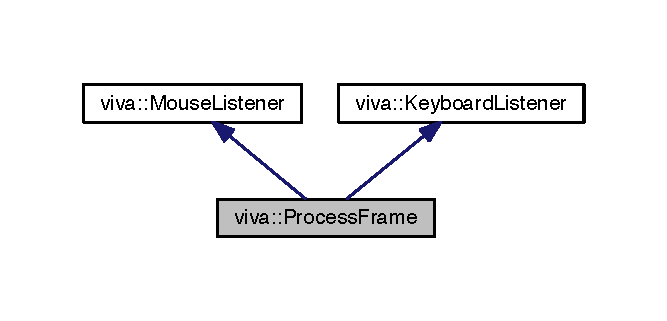
\includegraphics[width=320pt]{classviva_1_1_process_frame__inherit__graph}
\end{center}
\end{figure}


Collaboration diagram for viva\+:\+:Process\+Frame\+:
\nopagebreak
\begin{figure}[H]
\begin{center}
\leavevmode
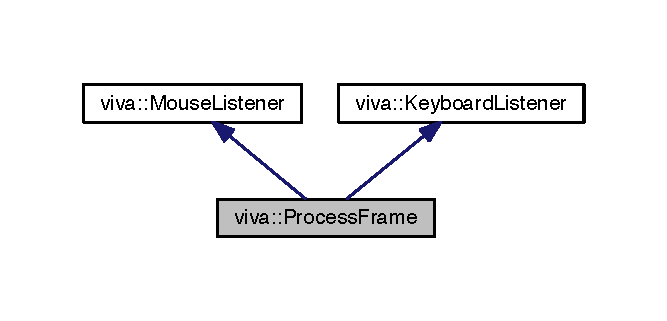
\includegraphics[width=320pt]{classviva_1_1_process_frame__coll__graph}
\end{center}
\end{figure}
\subsection*{Public Member Functions}
\begin{DoxyCompactItemize}
\item 
virtual void {\bfseries operator()} (const size\+\_\+t frameN, const Mat \&frame, Mat \&output)\hypertarget{classviva_1_1_process_frame_a82b5b1de63b91ce06fef1eff2d3fdf1e}{}\label{classviva_1_1_process_frame_a82b5b1de63b91ce06fef1eff2d3fdf1e}

\item 
virtual void \hyperlink{classviva_1_1_process_frame_a67f1444128085a4f18b6c7fe5086e6fc}{mouse\+Input} (int event, int x, int y, int flags)
\item 
virtual void \hyperlink{classviva_1_1_process_frame_a1d0476b4a6065fae4c0b46abf230be1c}{left\+Button\+Down} (int x, int y, int flags)
\item 
virtual void \hyperlink{classviva_1_1_process_frame_a03b8c90d990dcefdddf4ad735290d0eb}{right\+Button\+Down} (int x, int y, int flags)
\item 
virtual void \hyperlink{classviva_1_1_process_frame_a2c5155855fa6a88bb8124278ece845ee}{middle\+Button\+Down} (int x, int y, int flags)
\item 
virtual void \hyperlink{classviva_1_1_process_frame_a075654580641032ff792eedd3fd6b7a1}{mouse\+Move} (int x, int y, int flags)
\item 
virtual void \hyperlink{classviva_1_1_process_frame_a56d6805a983de9072ce31ea60688a408}{keyboard\+Input} (int key)
\end{DoxyCompactItemize}


\subsection{Detailed Description}
\hyperlink{classviva_1_1_process_frame}{Process\+Frame} functor interface accepting mouse and keyboard events 

\subsection{Member Function Documentation}
\index{viva\+::\+Process\+Frame@{viva\+::\+Process\+Frame}!keyboard\+Input@{keyboard\+Input}}
\index{keyboard\+Input@{keyboard\+Input}!viva\+::\+Process\+Frame@{viva\+::\+Process\+Frame}}
\subsubsection[{\texorpdfstring{keyboard\+Input(int key)}{keyboardInput(int key)}}]{\setlength{\rightskip}{0pt plus 5cm}virtual void viva\+::\+Process\+Frame\+::keyboard\+Input (
\begin{DoxyParamCaption}
\item[{int}]{key}
\end{DoxyParamCaption}
)\hspace{0.3cm}{\ttfamily [inline]}, {\ttfamily [virtual]}}\hypertarget{classviva_1_1_process_frame_a56d6805a983de9072ce31ea60688a408}{}\label{classviva_1_1_process_frame_a56d6805a983de9072ce31ea60688a408}
Inherited from Keyboard\+Listerner. Check \hyperlink{classviva_1_1_keyboard_listener}{Keyboard\+Listener} class for details. 

Reimplemented from \hyperlink{classviva_1_1_keyboard_listener_a903947e765f8130cfe1b3ce882c95998}{viva\+::\+Keyboard\+Listener}.

\index{viva\+::\+Process\+Frame@{viva\+::\+Process\+Frame}!left\+Button\+Down@{left\+Button\+Down}}
\index{left\+Button\+Down@{left\+Button\+Down}!viva\+::\+Process\+Frame@{viva\+::\+Process\+Frame}}
\subsubsection[{\texorpdfstring{left\+Button\+Down(int x, int y, int flags)}{leftButtonDown(int x, int y, int flags)}}]{\setlength{\rightskip}{0pt plus 5cm}virtual void viva\+::\+Process\+Frame\+::left\+Button\+Down (
\begin{DoxyParamCaption}
\item[{int}]{x, }
\item[{int}]{y, }
\item[{int}]{flags}
\end{DoxyParamCaption}
)\hspace{0.3cm}{\ttfamily [inline]}, {\ttfamily [virtual]}}\hypertarget{classviva_1_1_process_frame_a1d0476b4a6065fae4c0b46abf230be1c}{}\label{classviva_1_1_process_frame_a1d0476b4a6065fae4c0b46abf230be1c}
Inherited from \hyperlink{classviva_1_1_mouse_listener}{Mouse\+Listener}. Check \hyperlink{classviva_1_1_mouse_listener}{Mouse\+Listener} class for details 

Reimplemented from \hyperlink{classviva_1_1_mouse_listener_ae2b6952da67ea99e47f5fcfa2e1780c7}{viva\+::\+Mouse\+Listener}.

\index{viva\+::\+Process\+Frame@{viva\+::\+Process\+Frame}!middle\+Button\+Down@{middle\+Button\+Down}}
\index{middle\+Button\+Down@{middle\+Button\+Down}!viva\+::\+Process\+Frame@{viva\+::\+Process\+Frame}}
\subsubsection[{\texorpdfstring{middle\+Button\+Down(int x, int y, int flags)}{middleButtonDown(int x, int y, int flags)}}]{\setlength{\rightskip}{0pt plus 5cm}virtual void viva\+::\+Process\+Frame\+::middle\+Button\+Down (
\begin{DoxyParamCaption}
\item[{int}]{x, }
\item[{int}]{y, }
\item[{int}]{flags}
\end{DoxyParamCaption}
)\hspace{0.3cm}{\ttfamily [inline]}, {\ttfamily [virtual]}}\hypertarget{classviva_1_1_process_frame_a2c5155855fa6a88bb8124278ece845ee}{}\label{classviva_1_1_process_frame_a2c5155855fa6a88bb8124278ece845ee}
Inherited from \hyperlink{classviva_1_1_mouse_listener}{Mouse\+Listener}. Check \hyperlink{classviva_1_1_mouse_listener}{Mouse\+Listener} class for details 

Reimplemented from \hyperlink{classviva_1_1_mouse_listener_a3a61b77b23875e74f817020ee1603556}{viva\+::\+Mouse\+Listener}.

\index{viva\+::\+Process\+Frame@{viva\+::\+Process\+Frame}!mouse\+Input@{mouse\+Input}}
\index{mouse\+Input@{mouse\+Input}!viva\+::\+Process\+Frame@{viva\+::\+Process\+Frame}}
\subsubsection[{\texorpdfstring{mouse\+Input(int event, int x, int y, int flags)}{mouseInput(int event, int x, int y, int flags)}}]{\setlength{\rightskip}{0pt plus 5cm}virtual void viva\+::\+Process\+Frame\+::mouse\+Input (
\begin{DoxyParamCaption}
\item[{int}]{event, }
\item[{int}]{x, }
\item[{int}]{y, }
\item[{int}]{flags}
\end{DoxyParamCaption}
)\hspace{0.3cm}{\ttfamily [inline]}, {\ttfamily [virtual]}}\hypertarget{classviva_1_1_process_frame_a67f1444128085a4f18b6c7fe5086e6fc}{}\label{classviva_1_1_process_frame_a67f1444128085a4f18b6c7fe5086e6fc}
Inherited from \hyperlink{classviva_1_1_mouse_listener}{Mouse\+Listener}. Check \hyperlink{classviva_1_1_mouse_listener}{Mouse\+Listener} class for details 

Reimplemented from \hyperlink{classviva_1_1_mouse_listener_aba95f99370a82ae96f89fe9a1eebd00b}{viva\+::\+Mouse\+Listener}.

\index{viva\+::\+Process\+Frame@{viva\+::\+Process\+Frame}!mouse\+Move@{mouse\+Move}}
\index{mouse\+Move@{mouse\+Move}!viva\+::\+Process\+Frame@{viva\+::\+Process\+Frame}}
\subsubsection[{\texorpdfstring{mouse\+Move(int x, int y, int flags)}{mouseMove(int x, int y, int flags)}}]{\setlength{\rightskip}{0pt plus 5cm}virtual void viva\+::\+Process\+Frame\+::mouse\+Move (
\begin{DoxyParamCaption}
\item[{int}]{x, }
\item[{int}]{y, }
\item[{int}]{flags}
\end{DoxyParamCaption}
)\hspace{0.3cm}{\ttfamily [inline]}, {\ttfamily [virtual]}}\hypertarget{classviva_1_1_process_frame_a075654580641032ff792eedd3fd6b7a1}{}\label{classviva_1_1_process_frame_a075654580641032ff792eedd3fd6b7a1}
Inherited from \hyperlink{classviva_1_1_mouse_listener}{Mouse\+Listener}. Check \hyperlink{classviva_1_1_mouse_listener}{Mouse\+Listener} class for details 

Reimplemented from \hyperlink{classviva_1_1_mouse_listener_af48bb769c4935f52646567118cb05900}{viva\+::\+Mouse\+Listener}.

\index{viva\+::\+Process\+Frame@{viva\+::\+Process\+Frame}!right\+Button\+Down@{right\+Button\+Down}}
\index{right\+Button\+Down@{right\+Button\+Down}!viva\+::\+Process\+Frame@{viva\+::\+Process\+Frame}}
\subsubsection[{\texorpdfstring{right\+Button\+Down(int x, int y, int flags)}{rightButtonDown(int x, int y, int flags)}}]{\setlength{\rightskip}{0pt plus 5cm}virtual void viva\+::\+Process\+Frame\+::right\+Button\+Down (
\begin{DoxyParamCaption}
\item[{int}]{x, }
\item[{int}]{y, }
\item[{int}]{flags}
\end{DoxyParamCaption}
)\hspace{0.3cm}{\ttfamily [inline]}, {\ttfamily [virtual]}}\hypertarget{classviva_1_1_process_frame_a03b8c90d990dcefdddf4ad735290d0eb}{}\label{classviva_1_1_process_frame_a03b8c90d990dcefdddf4ad735290d0eb}
Inherited from \hyperlink{classviva_1_1_mouse_listener}{Mouse\+Listener}. Check \hyperlink{classviva_1_1_mouse_listener}{Mouse\+Listener} class for details 

Reimplemented from \hyperlink{classviva_1_1_mouse_listener_ae4a2d181ecebf2e4001ce6440339ed60}{viva\+::\+Mouse\+Listener}.



The documentation for this class was generated from the following file\+:\begin{DoxyCompactItemize}
\item 
viva.\+h\end{DoxyCompactItemize}

\hypertarget{classviva_1_1_process_input}{}\section{viva\+:\+:Process\+Input Class Reference}
\label{classviva_1_1_process_input}\index{viva\+::\+Process\+Input@{viva\+::\+Process\+Input}}
\subsection*{Public Member Functions}
\begin{DoxyCompactItemize}
\item 
{\bfseries Process\+Input} (Ptr$<$ \hyperlink{classviva_1_1_input}{Input} $>$ \&input, Ptr$<$ \hyperlink{classviva_1_1_buffered_channel}{Buffered\+Image\+Channel} $>$ \&channel)\hypertarget{classviva_1_1_process_input_a3c7834fde58d3864f0de2a4ef1f91242}{}\label{classviva_1_1_process_input_a3c7834fde58d3864f0de2a4ef1f91242}

\item 
void {\bfseries operator()} ()\hypertarget{classviva_1_1_process_input_a3c4525e0a526cf2e2df5ee934463bf9c}{}\label{classviva_1_1_process_input_a3c4525e0a526cf2e2df5ee934463bf9c}

\end{DoxyCompactItemize}


The documentation for this class was generated from the following files\+:\begin{DoxyCompactItemize}
\item 
viva.\+h\item 
viva.\+cpp\end{DoxyCompactItemize}

\hypertarget{classviva_1_1_processor}{}\section{viva\+:\+:Processor Class Reference}
\label{classviva_1_1_processor}\index{viva\+::\+Processor@{viva\+::\+Processor}}


{\ttfamily \#include $<$viva.\+h$>$}

\subsection*{Public Member Functions}
\begin{DoxyCompactItemize}
\item 
{\bfseries Processor} (int argc, const char $\ast$argv\mbox{[}$\,$\mbox{]})\hypertarget{classviva_1_1_processor_a353237f947a5441d3ca2fff1b5719b9d}{}\label{classviva_1_1_processor_a353237f947a5441d3ca2fff1b5719b9d}

\item 
void {\bfseries set\+Input\+Buffer\+Size} (size\+\_\+t size)\hypertarget{classviva_1_1_processor_a97dcc103d4fa72ea2de7949c816b959b}{}\label{classviva_1_1_processor_a97dcc103d4fa72ea2de7949c816b959b}

\item 
void {\bfseries set\+Output\+Buffer\+Size} (size\+\_\+t size)\hypertarget{classviva_1_1_processor_a21085a6e5c8bc297755ea50584624f2e}{}\label{classviva_1_1_processor_a21085a6e5c8bc297755ea50584624f2e}

\item 
void {\bfseries show\+Input} (bool show=true)\hypertarget{classviva_1_1_processor_a0856f185e561f03066755fd994892a9c}{}\label{classviva_1_1_processor_a0856f185e561f03066755fd994892a9c}

\item 
void {\bfseries show\+Time\+Info} (bool show=true)\hypertarget{classviva_1_1_processor_a5a5217ad1a90a00a26e991b161158e32}{}\label{classviva_1_1_processor_a5a5217ad1a90a00a26e991b161158e32}

\item 
void {\bfseries show\+Output} (bool show=true)\hypertarget{classviva_1_1_processor_ab6b872be8fae75cb1f70445d25f21481}{}\label{classviva_1_1_processor_ab6b872be8fae75cb1f70445d25f21481}

\item 
void {\bfseries set\+Input\+Window\+Name} (const string \&name)\hypertarget{classviva_1_1_processor_a1c7170ca5720762a5e4824215c10ed7e}{}\label{classviva_1_1_processor_a1c7170ca5720762a5e4824215c10ed7e}

\item 
void {\bfseries set\+Output\+Window\+Name} (const string \&name)\hypertarget{classviva_1_1_processor_a9e572aff063dfce565b53c4045c9ca1c}{}\label{classviva_1_1_processor_a9e572aff063dfce565b53c4045c9ca1c}

\item 
void {\bfseries set\+Input} (Ptr$<$ \hyperlink{classviva_1_1_input}{Input} $>$ \&input)\hypertarget{classviva_1_1_processor_a49d307c184c1f465ce472dd7c3d0d03e}{}\label{classviva_1_1_processor_a49d307c184c1f465ce472dd7c3d0d03e}

\item 
void {\bfseries set\+Output} (Ptr$<$ \hyperlink{classviva_1_1_output}{Output} $>$ \&output)\hypertarget{classviva_1_1_processor_a6411ad40ecad80d1585240c2583f5508}{}\label{classviva_1_1_processor_a6411ad40ecad80d1585240c2583f5508}

\item 
void {\bfseries listen\+To\+Mouse\+Events} ()\hypertarget{classviva_1_1_processor_a6467b7f49fbc075896823849a6b201ad}{}\label{classviva_1_1_processor_a6467b7f49fbc075896823849a6b201ad}

\item 
void {\bfseries listen\+To\+Keyboard\+Events} ()\hypertarget{classviva_1_1_processor_a9410f5f51eb4dd10f895db7502039760}{}\label{classviva_1_1_processor_a9410f5f51eb4dd10f895db7502039760}

\item 
void {\bfseries set\+Process} (Ptr$<$ \hyperlink{classviva_1_1_process_frame}{Process\+Frame} $>$ \&process)\hypertarget{classviva_1_1_processor_aab5f8e5a7b6f5356d11bbd39b1844440}{}\label{classviva_1_1_processor_aab5f8e5a7b6f5356d11bbd39b1844440}

\item 
void \hyperlink{classviva_1_1_processor_a9ab7ae5d6ed7720f94ee11e8b491dda2}{start\+Paused} ()
\item 
void \hyperlink{classviva_1_1_processor_a4c610fda2a3bf19feb7b7fd65b2ff6b0}{set\+Process} (function$<$ void(const size\+\_\+t frameN, const Mat \&frame, Mat \&output)$>$ functor)
\item 
void \hyperlink{classviva_1_1_processor_a073f5e9ea6a3557c217d67ab392e5852}{run} ()
\end{DoxyCompactItemize}


\subsection{Detailed Description}
\hyperlink{classviva_1_1_processor}{Processor} class. Entry point of a vivalib program We need to define an \hyperlink{classviva_1_1_input}{Input} , \hyperlink{classviva_1_1_process_frame}{Process\+Frame} and Output(optional) before starting to run a processor 

\subsection{Member Function Documentation}
\index{viva\+::\+Processor@{viva\+::\+Processor}!run@{run}}
\index{run@{run}!viva\+::\+Processor@{viva\+::\+Processor}}
\subsubsection[{\texorpdfstring{run()}{run()}}]{\setlength{\rightskip}{0pt plus 5cm}void Processor\+::run (
\begin{DoxyParamCaption}
{}
\end{DoxyParamCaption}
)}\hypertarget{classviva_1_1_processor_a073f5e9ea6a3557c217d67ab392e5852}{}\label{classviva_1_1_processor_a073f5e9ea6a3557c217d67ab392e5852}
Method to execute after defining the \hyperlink{classviva_1_1_processor}{Processor}\textquotesingle{}s \hyperlink{classviva_1_1_input}{Input}, \hyperlink{classviva_1_1_process_frame}{Process\+Frame}, and Output(optional) The input, process and output will run in three different threads and will comunicate using Buffed\+Channels between them. To exit you should press the E\+SC key. The S\+P\+A\+CE key will allow to pause and/or continue the video sequence \index{viva\+::\+Processor@{viva\+::\+Processor}!set\+Process@{set\+Process}}
\index{set\+Process@{set\+Process}!viva\+::\+Processor@{viva\+::\+Processor}}
\subsubsection[{\texorpdfstring{set\+Process(function$<$ void(const size\+\_\+t frame\+N, const Mat \&frame, Mat \&output)$>$ functor)}{setProcess(function< void(const size_t frameN, const Mat &frame, Mat &output)> functor)}}]{\setlength{\rightskip}{0pt plus 5cm}void viva\+::\+Processor\+::set\+Process (
\begin{DoxyParamCaption}
\item[{function$<$ void(const size\+\_\+t frameN, const Mat \&frame, Mat \&output)$>$}]{functor}
\end{DoxyParamCaption}
)\hspace{0.3cm}{\ttfamily [inline]}}\hypertarget{classviva_1_1_processor_a4c610fda2a3bf19feb7b7fd65b2ff6b0}{}\label{classviva_1_1_processor_a4c610fda2a3bf19feb7b7fd65b2ff6b0}
Set a process \index{viva\+::\+Processor@{viva\+::\+Processor}!start\+Paused@{start\+Paused}}
\index{start\+Paused@{start\+Paused}!viva\+::\+Processor@{viva\+::\+Processor}}
\subsubsection[{\texorpdfstring{start\+Paused()}{startPaused()}}]{\setlength{\rightskip}{0pt plus 5cm}void viva\+::\+Processor\+::start\+Paused (
\begin{DoxyParamCaption}
{}
\end{DoxyParamCaption}
)\hspace{0.3cm}{\ttfamily [inline]}}\hypertarget{classviva_1_1_processor_a9ab7ae5d6ed7720f94ee11e8b491dda2}{}\label{classviva_1_1_processor_a9ab7ae5d6ed7720f94ee11e8b491dda2}
Makes to pause the sequence at the fist frame. Waiting for the user to hit the S\+P\+A\+CE key in the keyboard to continue the execution of the sequence. It\textquotesingle{}s usefull when manual user selection is needed before running the algorithm 

The documentation for this class was generated from the following files\+:\begin{DoxyCompactItemize}
\item 
viva.\+h\item 
viva.\+cpp\end{DoxyCompactItemize}

\hypertarget{classviva_1_1_process_output}{}\section{viva\+:\+:Process\+Output Class Reference}
\label{classviva_1_1_process_output}\index{viva\+::\+Process\+Output@{viva\+::\+Process\+Output}}


{\ttfamily \#include $<$viva.\+h$>$}

\subsection*{Public Member Functions}
\begin{DoxyCompactItemize}
\item 
{\bfseries Process\+Output} (Ptr$<$ \hyperlink{classviva_1_1_output}{Output} $>$ \&output, Ptr$<$ \hyperlink{classviva_1_1_buffered_channel}{Buffered\+Image\+Channel} $>$ \&channel)\hypertarget{classviva_1_1_process_output_aa4a2cb166b42b1fa0cad620c0b5d7dd4}{}\label{classviva_1_1_process_output_aa4a2cb166b42b1fa0cad620c0b5d7dd4}

\item 
void {\bfseries operator()} ()\hypertarget{classviva_1_1_process_output_a1ff45ccbb3854063c62ca9fb098f0ea2}{}\label{classviva_1_1_process_output_a1ff45ccbb3854063c62ca9fb098f0ea2}

\end{DoxyCompactItemize}


\subsection{Detailed Description}
Parallel Processing \hyperlink{classviva_1_1_output}{Output} and communicating through the channel 

The documentation for this class was generated from the following files\+:\begin{DoxyCompactItemize}
\item 
viva.\+h\item 
viva.\+cpp\end{DoxyCompactItemize}

\hypertarget{classviva_1_1thread__guard}{}\section{viva\+:\+:thread\+\_\+guard Class Reference}
\label{classviva_1_1thread__guard}\index{viva\+::thread\+\_\+guard@{viva\+::thread\+\_\+guard}}


{\ttfamily \#include $<$viva.\+h$>$}

\subsection*{Public Member Functions}
\begin{DoxyCompactItemize}
\item 
{\bfseries thread\+\_\+guard} (std\+::thread \&t\+\_\+)\hypertarget{classviva_1_1thread__guard_a18469405edbe21f790ffced4f550e751}{}\label{classviva_1_1thread__guard_a18469405edbe21f790ffced4f550e751}

\item 
{\bfseries thread\+\_\+guard} (\hyperlink{classviva_1_1thread__guard}{thread\+\_\+guard} const \&)=delete\hypertarget{classviva_1_1thread__guard_a7f3d44c825af18f063b013f0623c2a48}{}\label{classviva_1_1thread__guard_a7f3d44c825af18f063b013f0623c2a48}

\item 
\hyperlink{classviva_1_1thread__guard}{thread\+\_\+guard} \& {\bfseries operator=} (\hyperlink{classviva_1_1thread__guard}{thread\+\_\+guard} const \&)=delete\hypertarget{classviva_1_1thread__guard_a001b0ac53f2bdc55ed74407dd43b1353}{}\label{classviva_1_1thread__guard_a001b0ac53f2bdc55ed74407dd43b1353}

\end{DoxyCompactItemize}


\subsection{Detailed Description}
Thread safe guard created to ensure all threads are joing when exiting their scope. 

The documentation for this class was generated from the following file\+:\begin{DoxyCompactItemize}
\item 
viva.\+h\end{DoxyCompactItemize}

\hypertarget{classviva_1_1_video_input}{}\section{viva\+:\+:Video\+Input Class Reference}
\label{classviva_1_1_video_input}\index{viva\+::\+Video\+Input@{viva\+::\+Video\+Input}}


{\ttfamily \#include $<$input.\+h$>$}



Inheritance diagram for viva\+:\+:Video\+Input\+:
\nopagebreak
\begin{figure}[H]
\begin{center}
\leavevmode
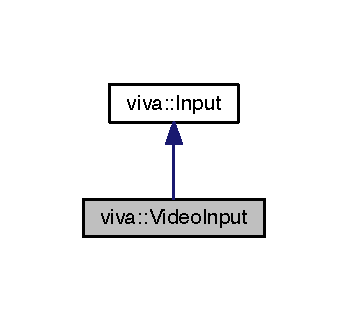
\includegraphics[width=167pt]{classviva_1_1_video_input__inherit__graph}
\end{center}
\end{figure}


Collaboration diagram for viva\+:\+:Video\+Input\+:
\nopagebreak
\begin{figure}[H]
\begin{center}
\leavevmode
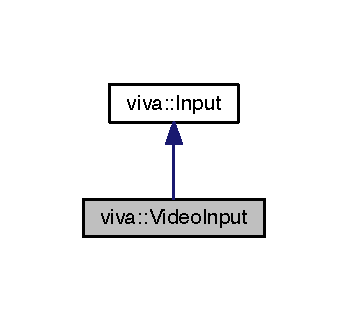
\includegraphics[width=167pt]{classviva_1_1_video_input__coll__graph}
\end{center}
\end{figure}
\subsection*{Public Member Functions}
\begin{DoxyCompactItemize}
\item 
\hyperlink{classviva_1_1_video_input_a37aabc4cd8ebc70dfa9b49bcb7a5d330}{Video\+Input} (const string \&filename, const Size \&size=Size(-\/1,-\/1), int color\+Flag=-\/1)
\item 
\hyperlink{classviva_1_1_video_input_adb9f341fb5b01b81b34f6f7f4f1eaa80}{Video\+Input} (const int id, const Size \&size=Size(-\/1,-\/1), int color\+Flag=-\/1)
\item 
\hyperlink{classviva_1_1_video_input_a88f06259f63094534518f32397024cfb}{Video\+Input} ()
\item 
\hyperlink{classviva_1_1_video_input_aece2200729baa8cef7db668583fb6470}{$\sim$\+Video\+Input} ()
\item 
bool \hyperlink{classviva_1_1_video_input_ab4819eb95ad41ba9a59536f60eefa5a9}{get\+Frame} (Mat \&frame)
\end{DoxyCompactItemize}
\subsection*{Protected Attributes}
\begin{DoxyCompactItemize}
\item 
Video\+Capture {\bfseries \+\_\+\+Camera\+Input}\hypertarget{classviva_1_1_video_input_a3b7196ebc0f6009f4ad63be661a00fd3}{}\label{classviva_1_1_video_input_a3b7196ebc0f6009f4ad63be661a00fd3}

\item 
bool {\bfseries \+\_\+opened}\hypertarget{classviva_1_1_video_input_ae98b3866cd376d0dfaf80b191c57db30}{}\label{classviva_1_1_video_input_ae98b3866cd376d0dfaf80b191c57db30}

\end{DoxyCompactItemize}


\subsection{Detailed Description}
Base class for Video Sequence inputs 

\subsection{Constructor \& Destructor Documentation}
\index{viva\+::\+Video\+Input@{viva\+::\+Video\+Input}!Video\+Input@{Video\+Input}}
\index{Video\+Input@{Video\+Input}!viva\+::\+Video\+Input@{viva\+::\+Video\+Input}}
\subsubsection[{\texorpdfstring{Video\+Input(const string \&filename, const Size \&size=\+Size(-\/1,-\/1), int color\+Flag=-\/1)}{VideoInput(const string &filename, const Size &size=Size(-1,-1), int colorFlag=-1)}}]{\setlength{\rightskip}{0pt plus 5cm}Video\+Input\+::\+Video\+Input (
\begin{DoxyParamCaption}
\item[{const string \&}]{filename, }
\item[{const Size \&}]{size = {\ttfamily Size(-\/1,-\/1)}, }
\item[{int}]{color\+Flag = {\ttfamily -\/1}}
\end{DoxyParamCaption}
)}\hypertarget{classviva_1_1_video_input_a37aabc4cd8ebc70dfa9b49bcb7a5d330}{}\label{classviva_1_1_video_input_a37aabc4cd8ebc70dfa9b49bcb7a5d330}
\hyperlink{classviva_1_1_video_input}{Video\+Input} constructor using a filename. 
\begin{DoxyParams}{Parameters}
{\em filename} & could be\+: 1)video file i.\+e., movie.\+avi 2)a regular pattern filename i.\+e. imag0\%2d.\+jpg 3)a url pointing to a video stream i.\+e., \href{http://domain.com/movie.avi}{\tt http\+://domain.\+com/movie.\+avi} \\
\hline
{\em size} & will scale the original feed to the desired size resolution unless (-\/1,-\/1) is defined \\
\hline
{\em color\+Flag} & Open\+CV conversion flag type value e.\+g., C\+V\+\_\+\+B\+G\+R2\+G\+R\+AY \\
\hline
\end{DoxyParams}
\index{viva\+::\+Video\+Input@{viva\+::\+Video\+Input}!Video\+Input@{Video\+Input}}
\index{Video\+Input@{Video\+Input}!viva\+::\+Video\+Input@{viva\+::\+Video\+Input}}
\subsubsection[{\texorpdfstring{Video\+Input(const int id, const Size \&size=\+Size(-\/1,-\/1), int color\+Flag=-\/1)}{VideoInput(const int id, const Size &size=Size(-1,-1), int colorFlag=-1)}}]{\setlength{\rightskip}{0pt plus 5cm}Video\+Input\+::\+Video\+Input (
\begin{DoxyParamCaption}
\item[{const int}]{id, }
\item[{const Size \&}]{size = {\ttfamily Size(-\/1,~-\/1)}, }
\item[{int}]{color\+Flag = {\ttfamily -\/1}}
\end{DoxyParamCaption}
)}\hypertarget{classviva_1_1_video_input_adb9f341fb5b01b81b34f6f7f4f1eaa80}{}\label{classviva_1_1_video_input_adb9f341fb5b01b81b34f6f7f4f1eaa80}
\hyperlink{classviva_1_1_video_input}{Video\+Input} constructor using a camera id. 
\begin{DoxyParams}{Parameters}
{\em id} & the camera identifier. \\
\hline
{\em size} & will scale the original feed to the desired size resolution unless (-\/1,-\/1) is defined \\
\hline
{\em color\+Flag} & Open\+CV conversion flag type value e.\+g., C\+V\+\_\+\+B\+G\+R2\+G\+R\+AY \\
\hline
\end{DoxyParams}
\index{viva\+::\+Video\+Input@{viva\+::\+Video\+Input}!Video\+Input@{Video\+Input}}
\index{Video\+Input@{Video\+Input}!viva\+::\+Video\+Input@{viva\+::\+Video\+Input}}
\subsubsection[{\texorpdfstring{Video\+Input()}{VideoInput()}}]{\setlength{\rightskip}{0pt plus 5cm}Video\+Input\+::\+Video\+Input (
\begin{DoxyParamCaption}
{}
\end{DoxyParamCaption}
)}\hypertarget{classviva_1_1_video_input_a88f06259f63094534518f32397024cfb}{}\label{classviva_1_1_video_input_a88f06259f63094534518f32397024cfb}
Default constructor \index{viva\+::\+Video\+Input@{viva\+::\+Video\+Input}!````~Video\+Input@{$\sim$\+Video\+Input}}
\index{````~Video\+Input@{$\sim$\+Video\+Input}!viva\+::\+Video\+Input@{viva\+::\+Video\+Input}}
\subsubsection[{\texorpdfstring{$\sim$\+Video\+Input()}{~VideoInput()}}]{\setlength{\rightskip}{0pt plus 5cm}Video\+Input\+::$\sim$\+Video\+Input (
\begin{DoxyParamCaption}
{}
\end{DoxyParamCaption}
)}\hypertarget{classviva_1_1_video_input_aece2200729baa8cef7db668583fb6470}{}\label{classviva_1_1_video_input_aece2200729baa8cef7db668583fb6470}
Desctructor 

\subsection{Member Function Documentation}
\index{viva\+::\+Video\+Input@{viva\+::\+Video\+Input}!get\+Frame@{get\+Frame}}
\index{get\+Frame@{get\+Frame}!viva\+::\+Video\+Input@{viva\+::\+Video\+Input}}
\subsubsection[{\texorpdfstring{get\+Frame(\+Mat \&frame)}{getFrame(Mat &frame)}}]{\setlength{\rightskip}{0pt plus 5cm}bool Video\+Input\+::get\+Frame (
\begin{DoxyParamCaption}
\item[{Mat \&}]{frame}
\end{DoxyParamCaption}
)\hspace{0.3cm}{\ttfamily [virtual]}}\hypertarget{classviva_1_1_video_input_ab4819eb95ad41ba9a59536f60eefa5a9}{}\label{classviva_1_1_video_input_ab4819eb95ad41ba9a59536f60eefa5a9}
Overrided from \hyperlink{classviva_1_1_input}{Input} Base Class. Used to extract a frame from the input sequence. Returns whether or not a frame was sucessfuly returned. 
\begin{DoxyParams}{Parameters}
{\em frame} & output image frame from the sequence \\
\hline
\end{DoxyParams}


Implements \hyperlink{classviva_1_1_input_aa24f1c290895fba92d7e1c6032dc4ecb}{viva\+::\+Input}.



The documentation for this class was generated from the following files\+:\begin{DoxyCompactItemize}
\item 
input.\+h\item 
input.\+cpp\end{DoxyCompactItemize}

\hypertarget{classviva_1_1_video_output}{}\section{viva\+:\+:Video\+Output Class Reference}
\label{classviva_1_1_video_output}\index{viva\+::\+Video\+Output@{viva\+::\+Video\+Output}}


{\ttfamily \#include $<$output.\+h$>$}



Inheritance diagram for viva\+:\+:Video\+Output\+:
\nopagebreak
\begin{figure}[H]
\begin{center}
\leavevmode
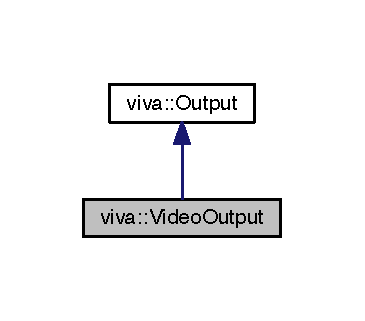
\includegraphics[width=175pt]{classviva_1_1_video_output__inherit__graph}
\end{center}
\end{figure}


Collaboration diagram for viva\+:\+:Video\+Output\+:
\nopagebreak
\begin{figure}[H]
\begin{center}
\leavevmode
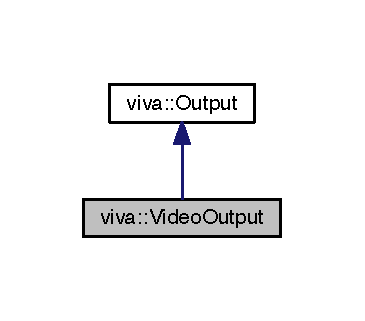
\includegraphics[width=175pt]{classviva_1_1_video_output__coll__graph}
\end{center}
\end{figure}
\subsection*{Public Member Functions}
\begin{DoxyCompactItemize}
\item 
\hyperlink{classviva_1_1_video_output_af696901783add61a8855e325d214db88}{Video\+Output} (const string \&filename, Size size=Size(-\/1,-\/1), int fps=30, C\+O\+D\+EC codec=C\+O\+D\+E\+C\+::\+M\+P\+E\+G4, int code\+Flag=-\/1)
\item 
virtual bool \hyperlink{classviva_1_1_video_output_ae18c0d361f077619db8d3cdab8283697}{write\+Frame} (Mat \&frame)
\item 
void \hyperlink{classviva_1_1_video_output_a261b56ddf7128f672adf880f6788798e}{set\+Codec} (C\+O\+D\+EC codec)
\item 
\hyperlink{classviva_1_1_video_output_af8cd62606fabbf14b33f1625cf1d2cb6}{$\sim$\+Video\+Output} ()
\end{DoxyCompactItemize}
\subsection*{Additional Inherited Members}


\subsection{Detailed Description}
Video \hyperlink{classviva_1_1_output}{Output} class. Generates a video file using an specified coded, resolution, frame per second rate and conversionflag 

\subsection{Constructor \& Destructor Documentation}
\index{viva\+::\+Video\+Output@{viva\+::\+Video\+Output}!Video\+Output@{Video\+Output}}
\index{Video\+Output@{Video\+Output}!viva\+::\+Video\+Output@{viva\+::\+Video\+Output}}
\subsubsection[{\texorpdfstring{Video\+Output(const string \&filename, Size size=\+Size(-\/1,-\/1), int fps=30, C\+O\+D\+E\+C codec=\+C\+O\+D\+E\+C\+::\+M\+P\+E\+G4, int code\+Flag=-\/1)}{VideoOutput(const string &filename, Size size=Size(-1,-1), int fps=30, CODEC codec=CODEC::MPEG4, int codeFlag=-1)}}]{\setlength{\rightskip}{0pt plus 5cm}Video\+Output\+::\+Video\+Output (
\begin{DoxyParamCaption}
\item[{const string \&}]{filename, }
\item[{Size}]{size = {\ttfamily Size(-\/1,-\/1)}, }
\item[{int}]{fps = {\ttfamily 30}, }
\item[{C\+O\+D\+EC}]{codec = {\ttfamily CODEC\+:\+:MPEG4}, }
\item[{int}]{code\+Flag = {\ttfamily -\/1}}
\end{DoxyParamCaption}
)}\hypertarget{classviva_1_1_video_output_af696901783add61a8855e325d214db88}{}\label{classviva_1_1_video_output_af696901783add61a8855e325d214db88}
Creates a Video \hyperlink{classviva_1_1_output}{Output} using the 
\begin{DoxyParams}{Parameters}
{\em filename} & video file filename \\
\hline
{\em size} & scale the final video output to the desired resolution \\
\hline
{\em fps} & frame per seconds \\
\hline
{\em codec} & One of the available Open\+CV codecs installed in your computer \\
\hline
{\em code\+Flag} & color conversion e.\+g., C\+V\+\_\+\+B\+G\+R2\+G\+R\+AY \\
\hline
\end{DoxyParams}
\index{viva\+::\+Video\+Output@{viva\+::\+Video\+Output}!````~Video\+Output@{$\sim$\+Video\+Output}}
\index{````~Video\+Output@{$\sim$\+Video\+Output}!viva\+::\+Video\+Output@{viva\+::\+Video\+Output}}
\subsubsection[{\texorpdfstring{$\sim$\+Video\+Output()}{~VideoOutput()}}]{\setlength{\rightskip}{0pt plus 5cm}viva\+::\+Video\+Output\+::$\sim$\+Video\+Output (
\begin{DoxyParamCaption}
{}
\end{DoxyParamCaption}
)\hspace{0.3cm}{\ttfamily [inline]}}\hypertarget{classviva_1_1_video_output_af8cd62606fabbf14b33f1625cf1d2cb6}{}\label{classviva_1_1_video_output_af8cd62606fabbf14b33f1625cf1d2cb6}
Destructor will release the Video\+Writer output 

\subsection{Member Function Documentation}
\index{viva\+::\+Video\+Output@{viva\+::\+Video\+Output}!set\+Codec@{set\+Codec}}
\index{set\+Codec@{set\+Codec}!viva\+::\+Video\+Output@{viva\+::\+Video\+Output}}
\subsubsection[{\texorpdfstring{set\+Codec(\+C\+O\+D\+E\+C codec)}{setCodec(CODEC codec)}}]{\setlength{\rightskip}{0pt plus 5cm}void viva\+::\+Video\+Output\+::set\+Codec (
\begin{DoxyParamCaption}
\item[{C\+O\+D\+EC}]{codec}
\end{DoxyParamCaption}
)\hspace{0.3cm}{\ttfamily [inline]}}\hypertarget{classviva_1_1_video_output_a261b56ddf7128f672adf880f6788798e}{}\label{classviva_1_1_video_output_a261b56ddf7128f672adf880f6788798e}
Set the codec to use while generating the video file \index{viva\+::\+Video\+Output@{viva\+::\+Video\+Output}!write\+Frame@{write\+Frame}}
\index{write\+Frame@{write\+Frame}!viva\+::\+Video\+Output@{viva\+::\+Video\+Output}}
\subsubsection[{\texorpdfstring{write\+Frame(\+Mat \&frame)}{writeFrame(Mat &frame)}}]{\setlength{\rightskip}{0pt plus 5cm}bool Video\+Output\+::write\+Frame (
\begin{DoxyParamCaption}
\item[{Mat \&}]{frame}
\end{DoxyParamCaption}
)\hspace{0.3cm}{\ttfamily [virtual]}}\hypertarget{classviva_1_1_video_output_ae18c0d361f077619db8d3cdab8283697}{}\label{classviva_1_1_video_output_ae18c0d361f077619db8d3cdab8283697}
Override from \hyperlink{classviva_1_1_output}{Output} base class 

Implements \hyperlink{classviva_1_1_output_ac74a311b4d151c5507d1351b7fc3426e}{viva\+::\+Output}.



The documentation for this class was generated from the following files\+:\begin{DoxyCompactItemize}
\item 
output.\+h\item 
output.\+cpp\end{DoxyCompactItemize}

%--- End generated contents ---

% Index
\backmatter
\newpage
\phantomsection
\clearemptydoublepage
\addcontentsline{toc}{chapter}{Index}
\printindex

\end{document}
